\section{Asymmetry Extraction}
As mentioned before, hadrons from different hemispheres constitute hadron pairs and each hadron has a Collins angle $\phi$. Now with the selected particles, hadron pairs can be constructed and Collins angle distribution can be analyzed. %Fig.~\ref{fig:pipiP0phi} shows examples of the Collins angle $\phi_1+\phi_2$ of $\pi^0\pi^+$ pairs. 

Double ratio method has been discussed in section~\ref{sec:observable}. Here in section~\ref{sec:resutlsfrommc} the false asymmetries after using double ratio method are examined using MC. Section~\ref{sec:resultsfromexp} shows asymmetries of experiment data. 

\subsection{Results from Simulation}
\label{sec:resutlsfrommc}
Before moving to asymmetry measurement for experiment data, a test to examine the behavior of all constraints is necessary. Monte Carlo does not have Collins effect input so the double ratio asymmetry should be 0. However, the detector acceptance may generate a dependence of the data on the azimuthal angle $\phi$ similar to the dependence caused by the Collins effect to be measured as shown in Fig.~\ref{fig:differentthetarange} and lead to false asymmetries. Fiducial cuts make this effect smaller but it does not disappear. Double ratio method then cancels most as well as the cosine modulations caused by boson radiation and the remaining is estimated by simulations and we call it false asymmetry.
\begin{figure}[H]
    \centering
    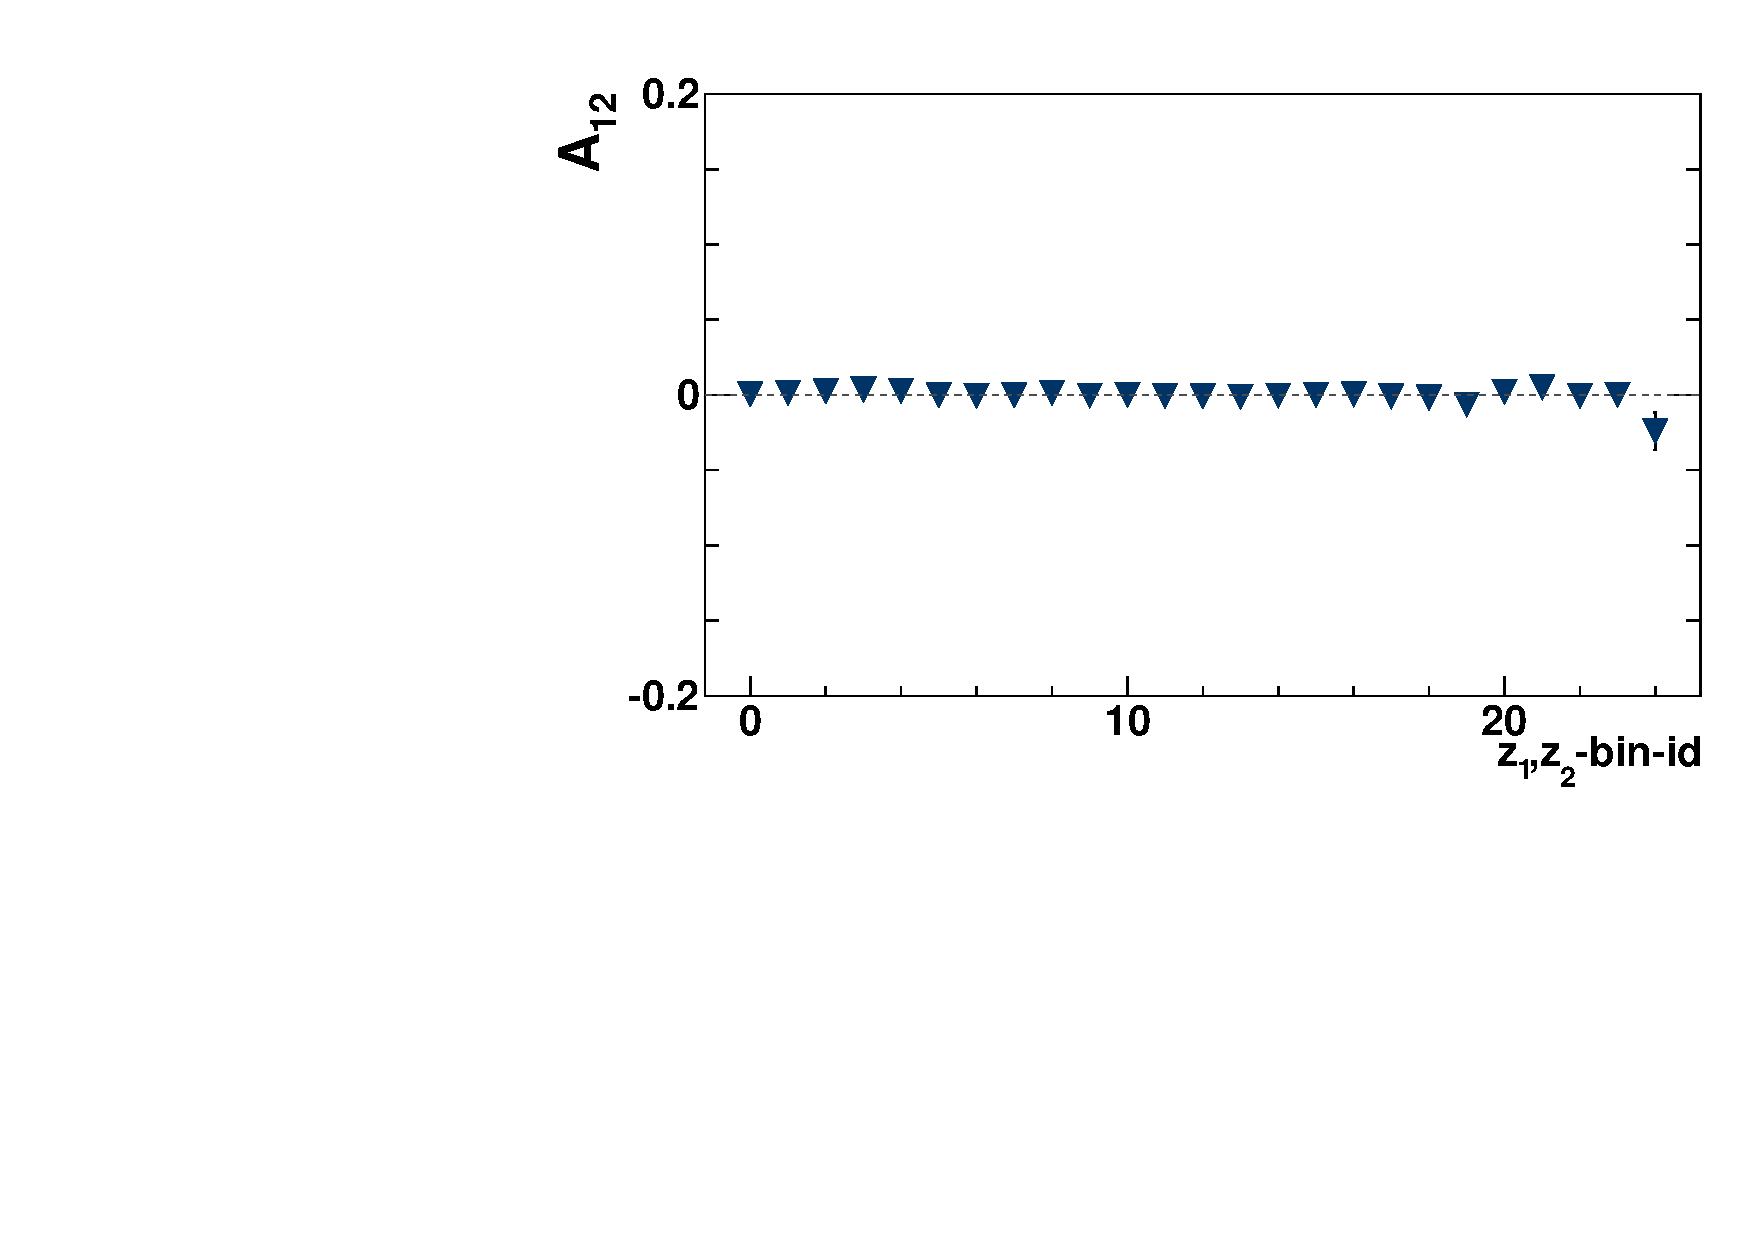
\includegraphics[width=0.6\textwidth,natwidth=250,natheight=100]{figure_asy/ComZ_Phi12_pi0.pdf}
    \caption{$(z_1,z_{2})$ bins asymmetry measured with MC data.}
    \label{fig:mc_example}
\end{figure}
The $\cos$ fit of MC simulation data shows negligible amplitude as shown in Fig.~\ref{fig:mc_example} and this amplitude together with the uncertainty will contribute to the one-sided systematic uncertainties, namely the asymmetric maximum deviation from zero.   

\subsection{Results from Experimental Data}
\label{sec:resultsfromexp}
\subsubsection{\texorpdfstring{Raw Asymmetry of $\pi^0$ and $\eta$}{Raw Asymmetry of pi0 and eta}}
Data used in this study contains Belle experiments from 7 to 73. In Fig.~\ref{fig:exp_pi0_result}, significant nonzero asymmetries can be observed. The left and right upper plots are $z_1$ bins and $P_{t1}$ bins results. A clear increasing pattern can be observed, namely the higher $z$/$P_t$ bin the higher asymmetry and this is consistent with previous results in \cite{ChargedPionResult2}\cite{ChargedPionResult}.

The combined bins have a more complicated pattern. Remember that in Fig.~\ref{fig:z1z2binning} , the first five combined bins contain one lowest $z$ hadron with another same or higher $z$ hadron. Thus the asymmetries of first four bins are increasing and form the first tier of $(z_1,z_2)$ bins. Combined bins 5 to 7 contain the second lowest $z$ together with another same or higher $z$ hadron and form the second tier. The asymmetry of the fifth bin is lower than fourth bin, because the fourth bin contains hadrons with one highest and one lowest $z$ while the fifth bin only contains hadrons with second lowest $z$. Start from fifth bin, the next three bins' asymmetries are increasing. The last 3 bins behave just like the middle 3 bins, but with higher asymmetries. 

In Fig.~\ref{fig:pt1pt2binning} $(P_{t1},P_{t2})$ bin have the same term structure with $(z_1,z_2)$ bin, and the asymmetry shows similar pattern. 
\begin{figure}[H]
  \centering     
    \subfigure[$\pi^0$ $z_1$ bins asymmetry]{\label{fig:exp_singlez}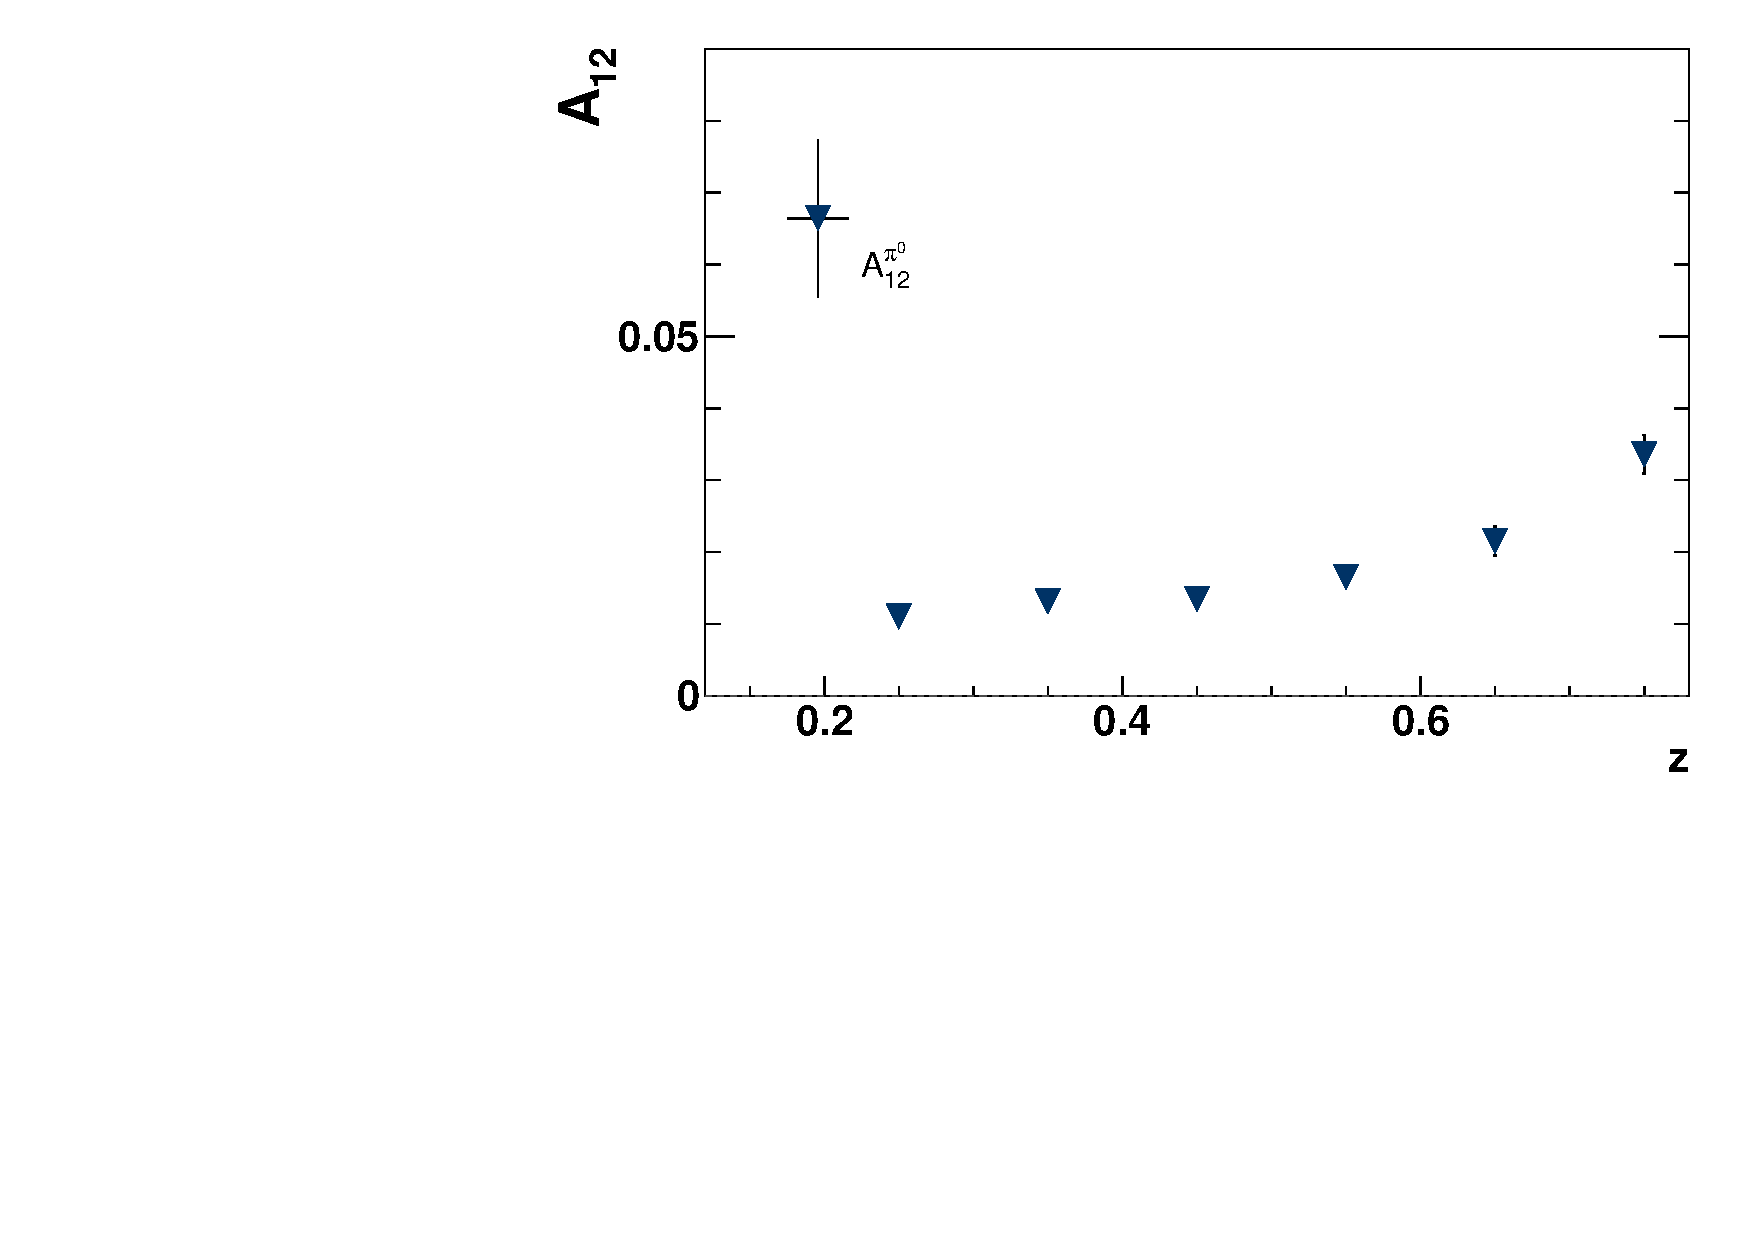
\includegraphics[width=.49\textwidth,natwidth=800,natheight=600]{figure_asy/Pi0NoCorrection0.pdf}}
 \subfigure[$\pi^0$ $P_{t1}$ bins asymmetry]{\label{fig:exp_singlez1}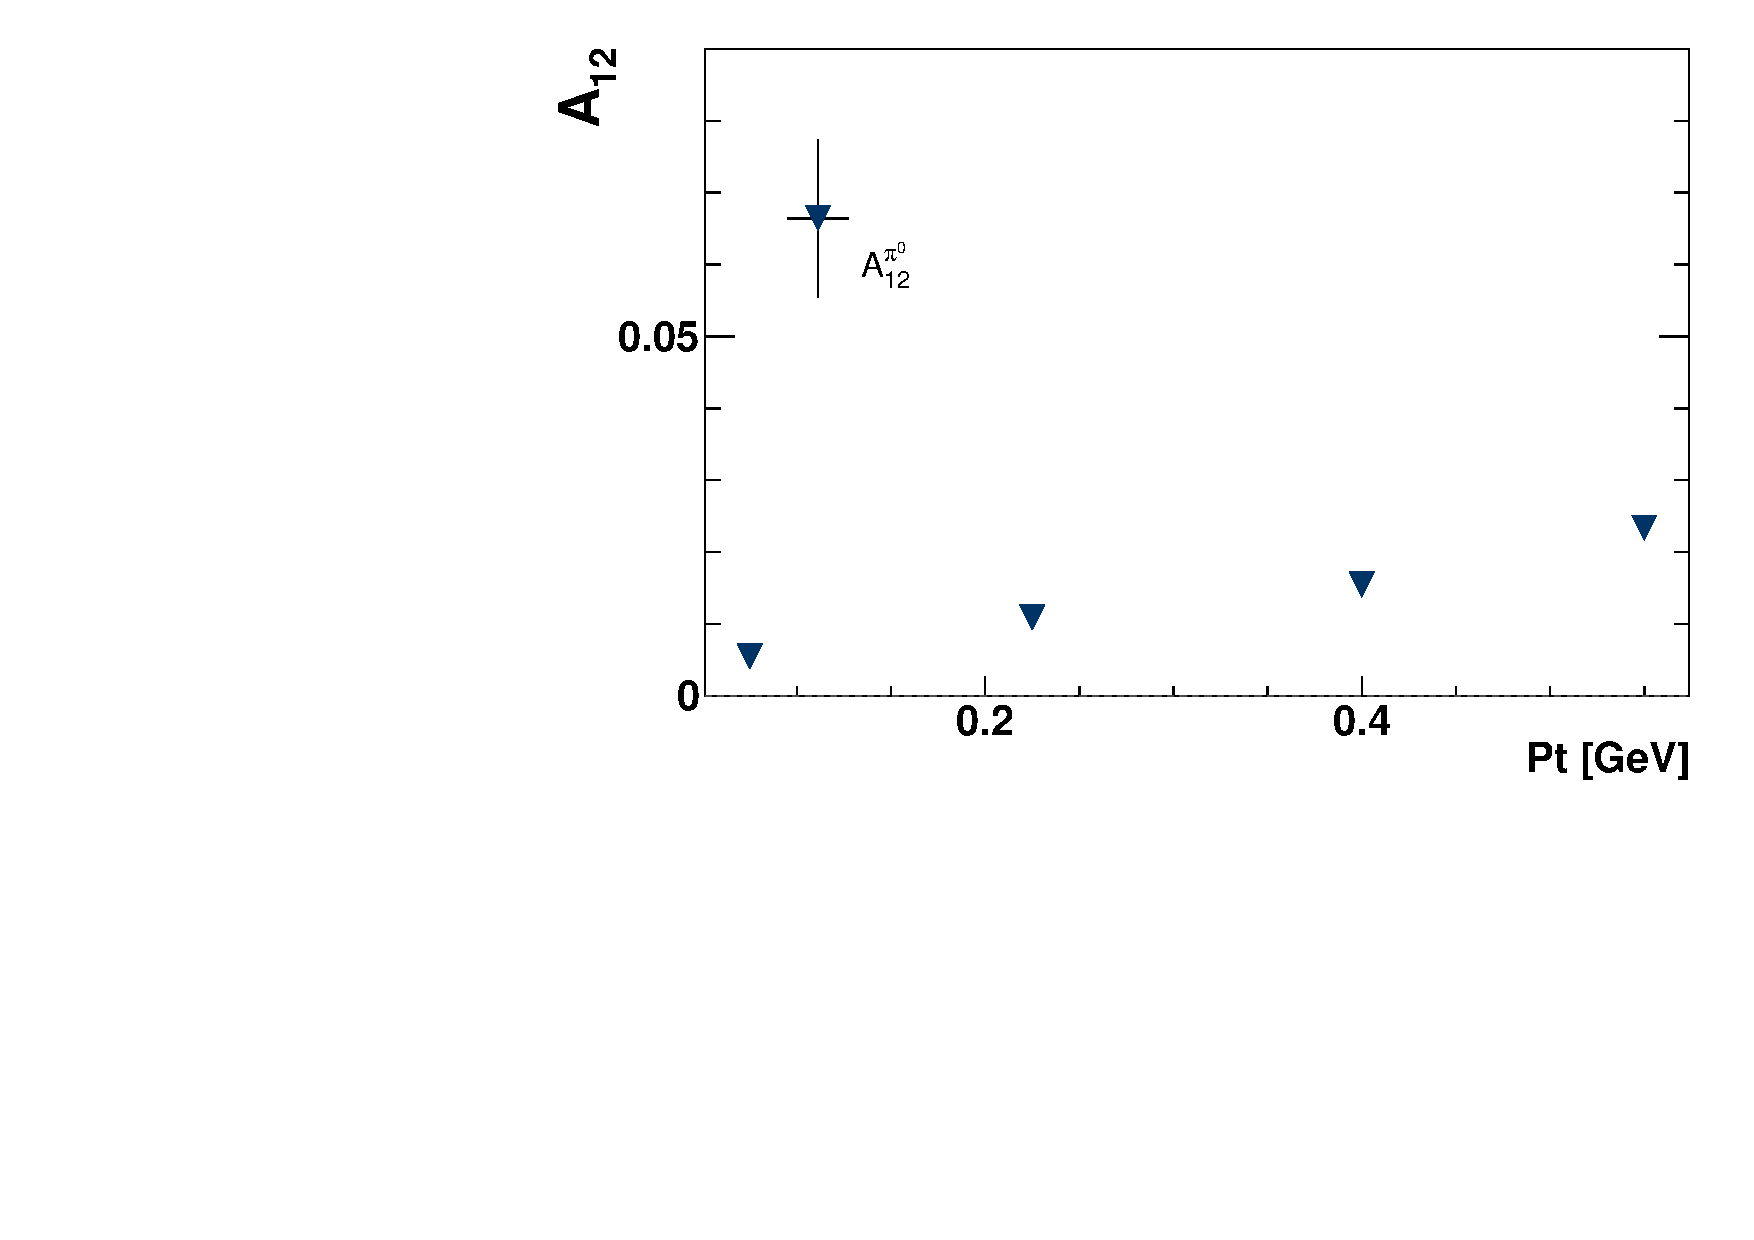
\includegraphics[width=.49\textwidth,natwidth=800,natheight=600]{figure_asy/Pi0NoCorrection2.pdf}}
  \subfigure[$\pi^0$ $(z_1,z_2)$ bins asymmetry]{\label{fig:exp_singlept}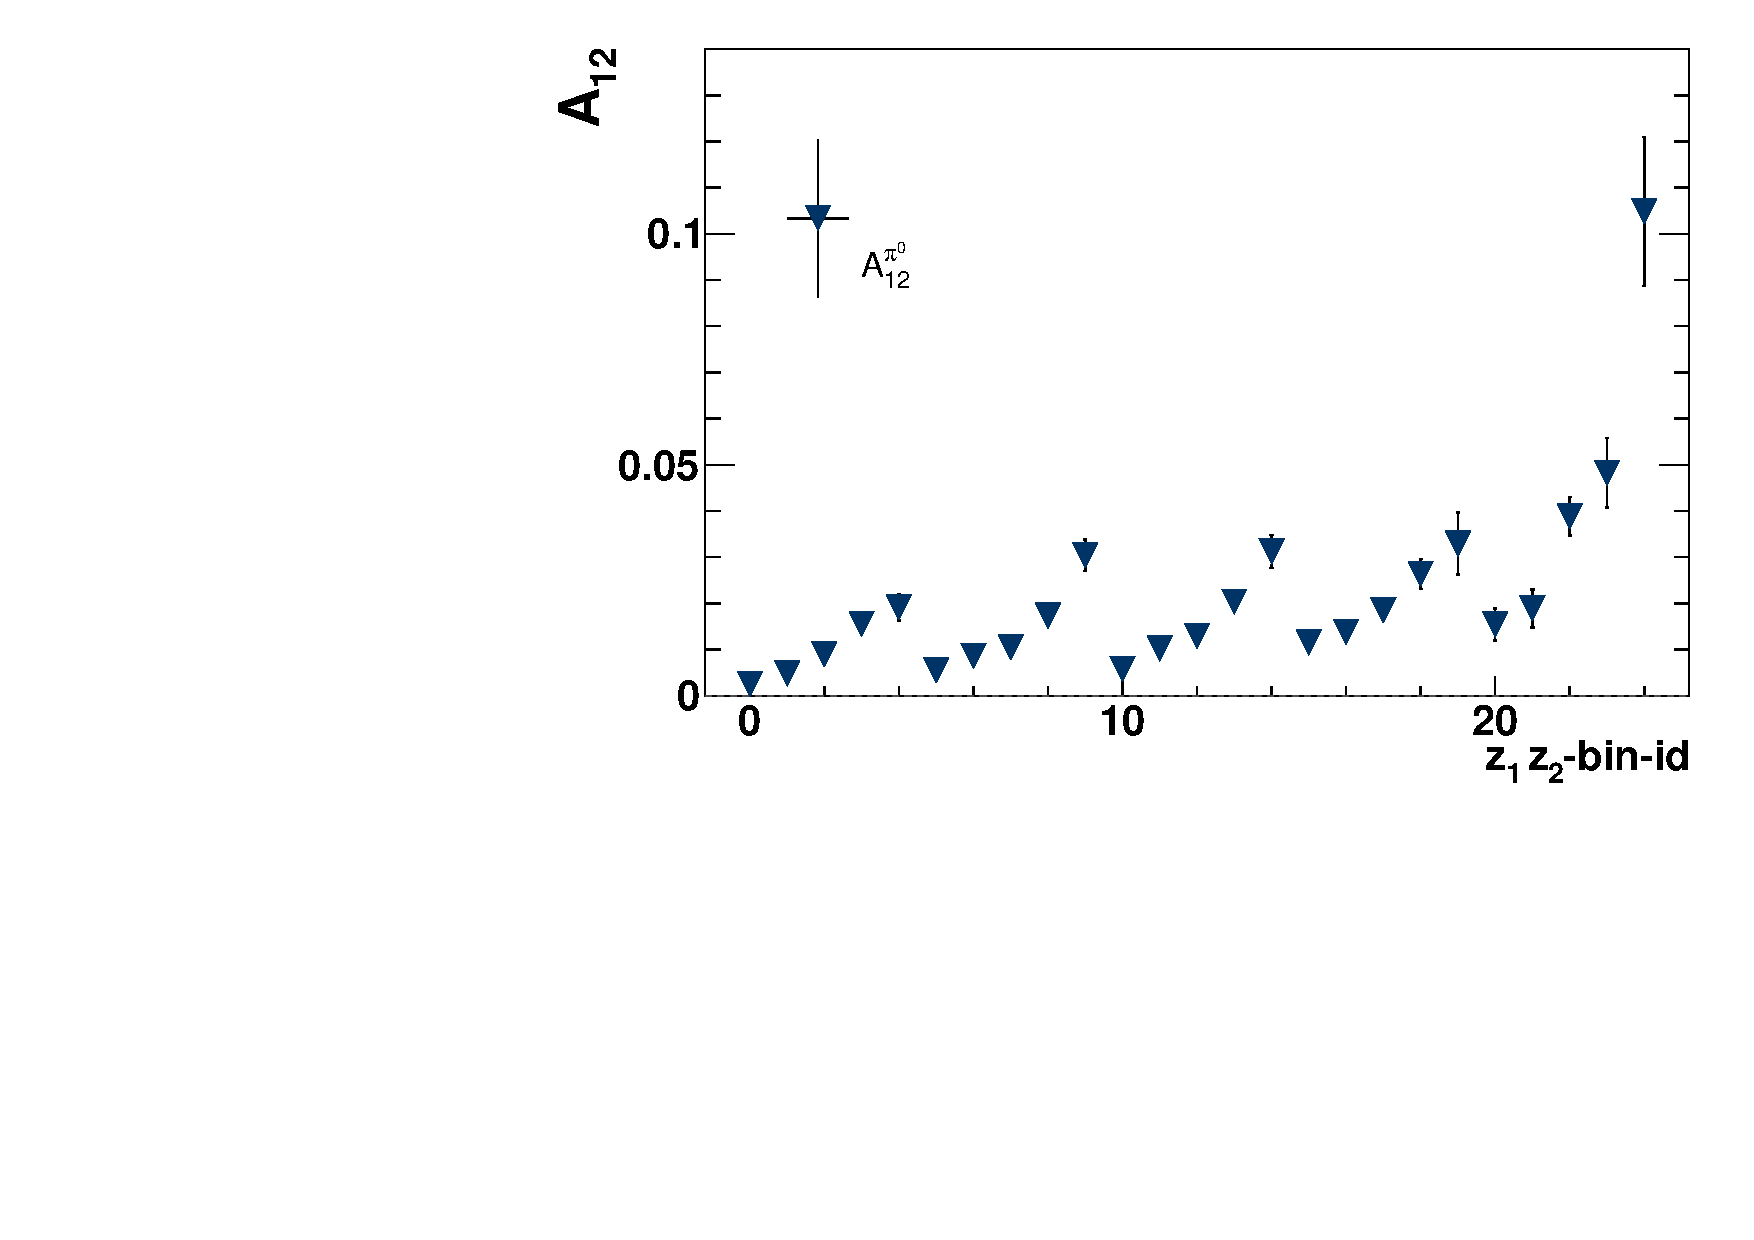
\includegraphics[width=.49\textwidth,natwidth=800,natheight=600]{figure_asy/Pi0NoCorrection1.pdf}}
  \subfigure[$\pi^0$ $(P_{t1},P_{t2})$ bins asymmetry]{\label{fig:exp_singlept1}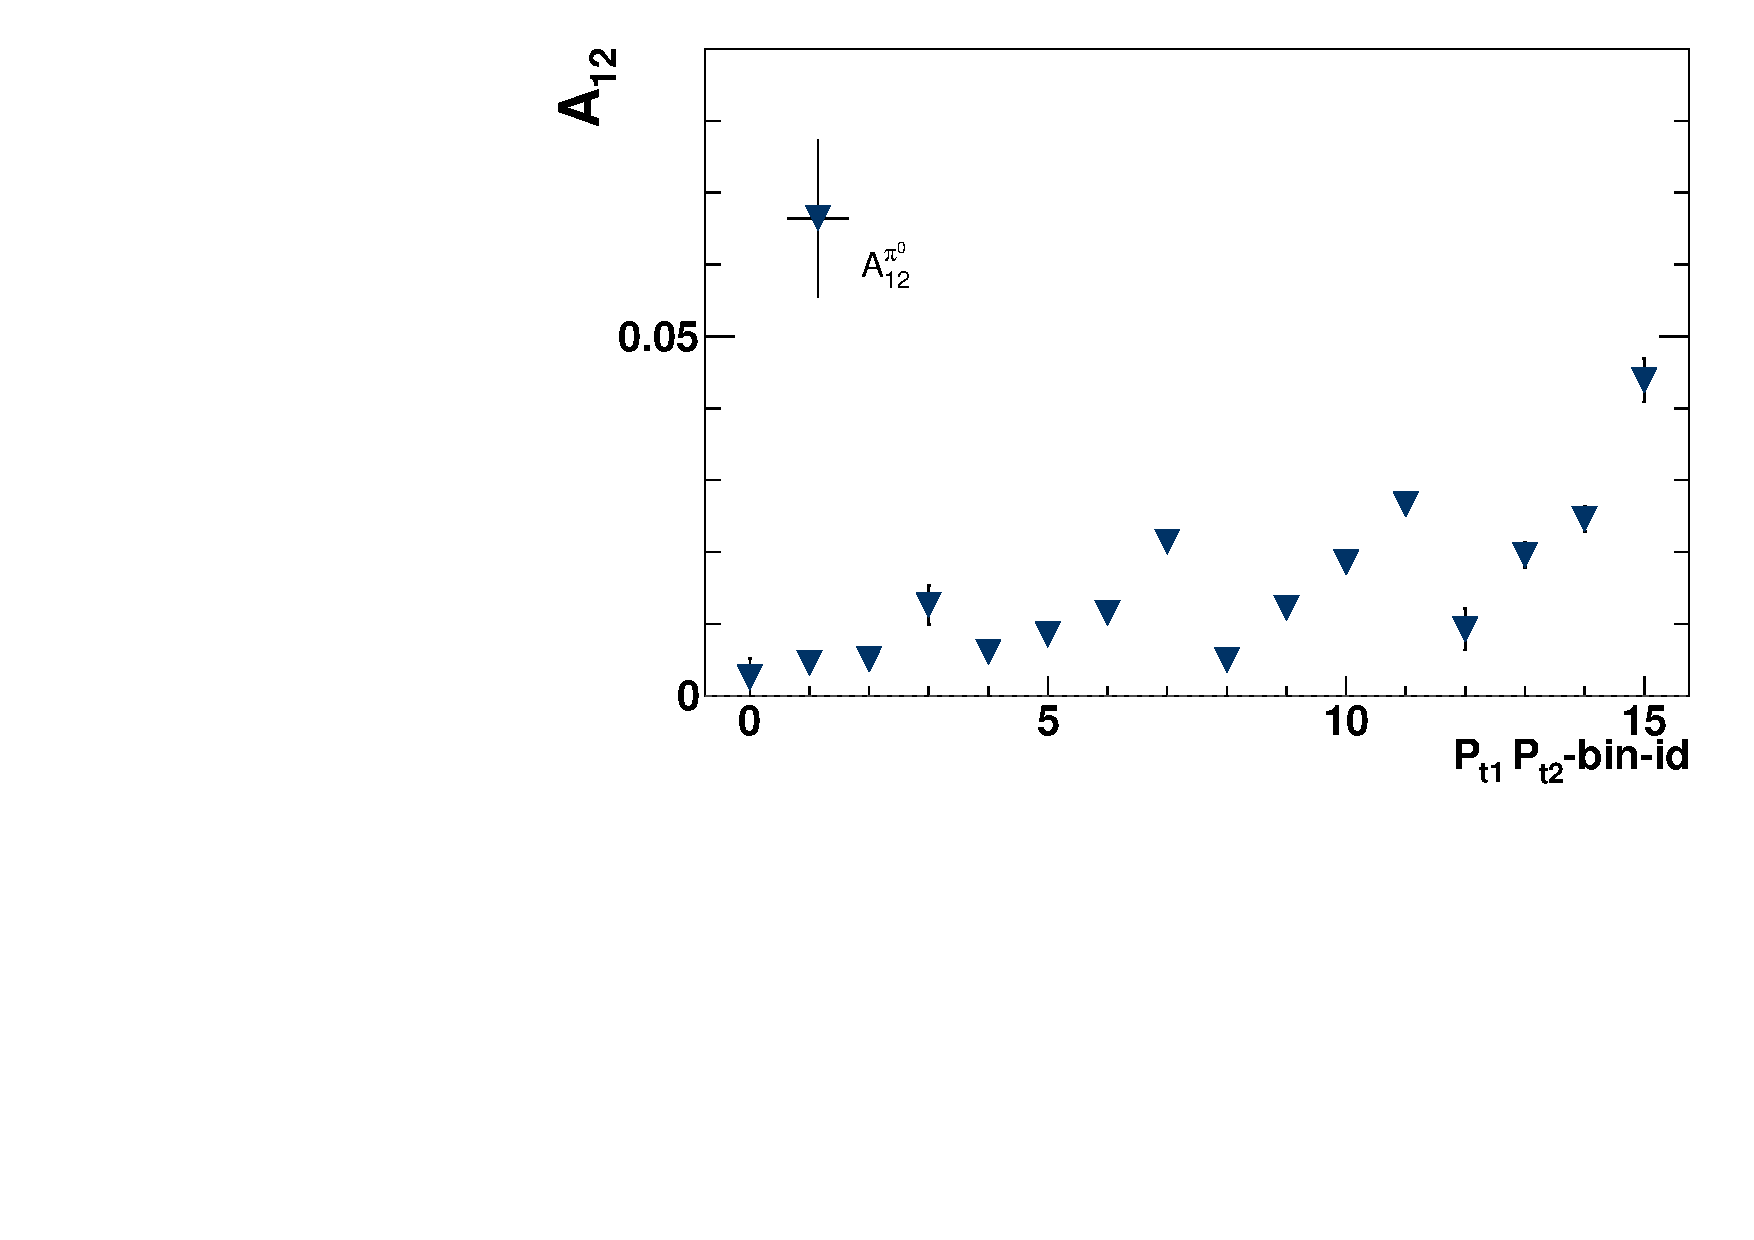
\includegraphics[width=.49\textwidth,natwidth=800,natheight=600]{figure_asy/Pi0NoCorrection3.pdf}}
  \caption{Experiment $\pi^0$ double ratio asymmetry $\nicefrac{A^{0\pm}_{12}}{A^L_{12}}$}
  \label{fig:exp_pi0_result}
\end{figure}

In Fig.~\ref{fig:exp_eta_result} the constraint $z> 0.3$ is applied to all double ratios containing $\eta$ mesons. Fig.~\ref{fig:exp_eta_result} shows positive asymmetry. As the statistics are lower, the error bars are larger than $\pi^0$. The difference of $\eta$ and $\pi^0$ is of interest because the Collins asymmetry may explain the larger transverse single spin asymmetry of $\eta$ observed in $pp$ collision \cite{StarTSSA1}\cite{StarTSSA2}. Also $\eta$ has strange quark and this new flavor may cause difference between $\pi^0$ and $\eta$.
 
\begin{figure}[H]
  \centering     
  \subfigure[$\eta$ $z_1$ bins asymmetry]{\label{fig:exp_singlez_eta}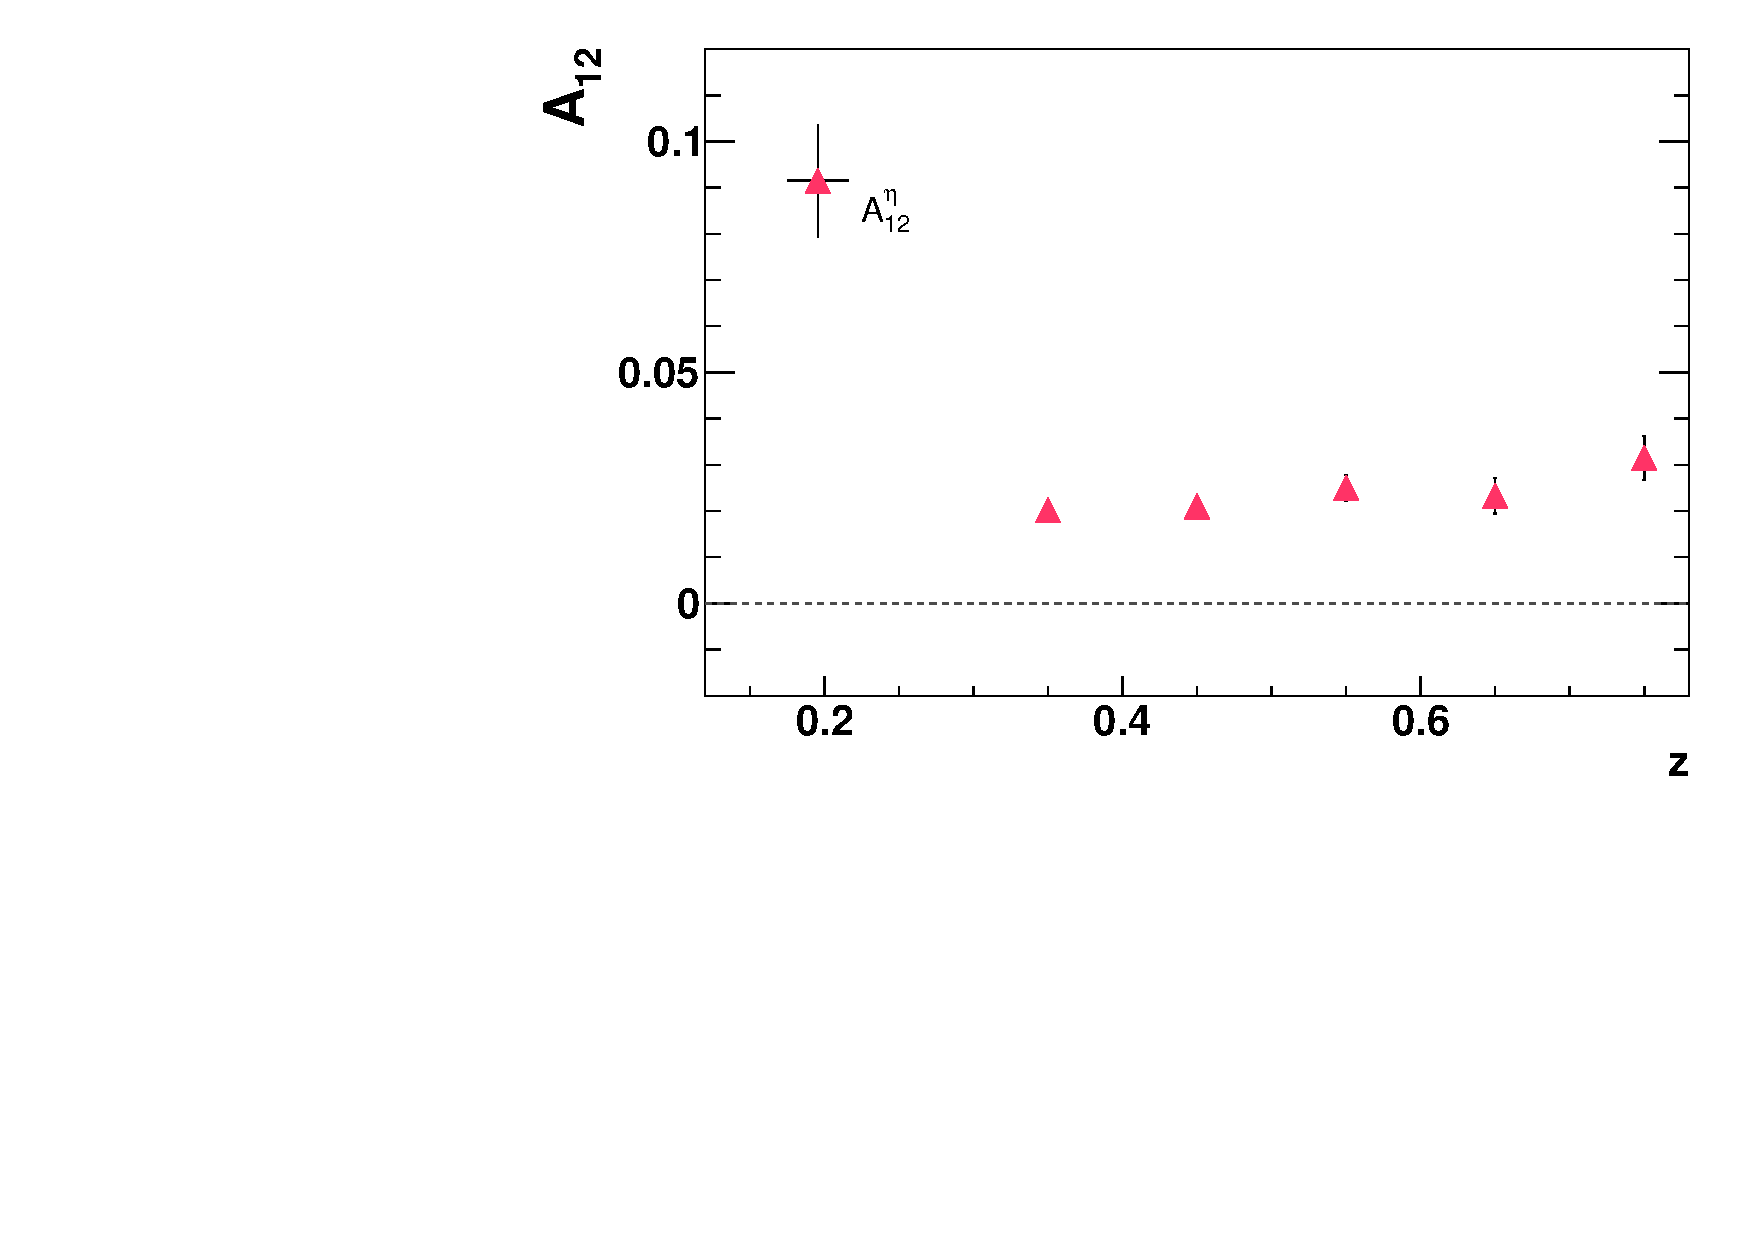
\includegraphics[width=.48\textwidth,natwidth=600,natheight=400]{figure_asy/EtaNoCorrection0.pdf}}
  \subfigure[$\eta$ $P_{t1}$ bins asymmetry]{\label{fig:exp_comz1_eta}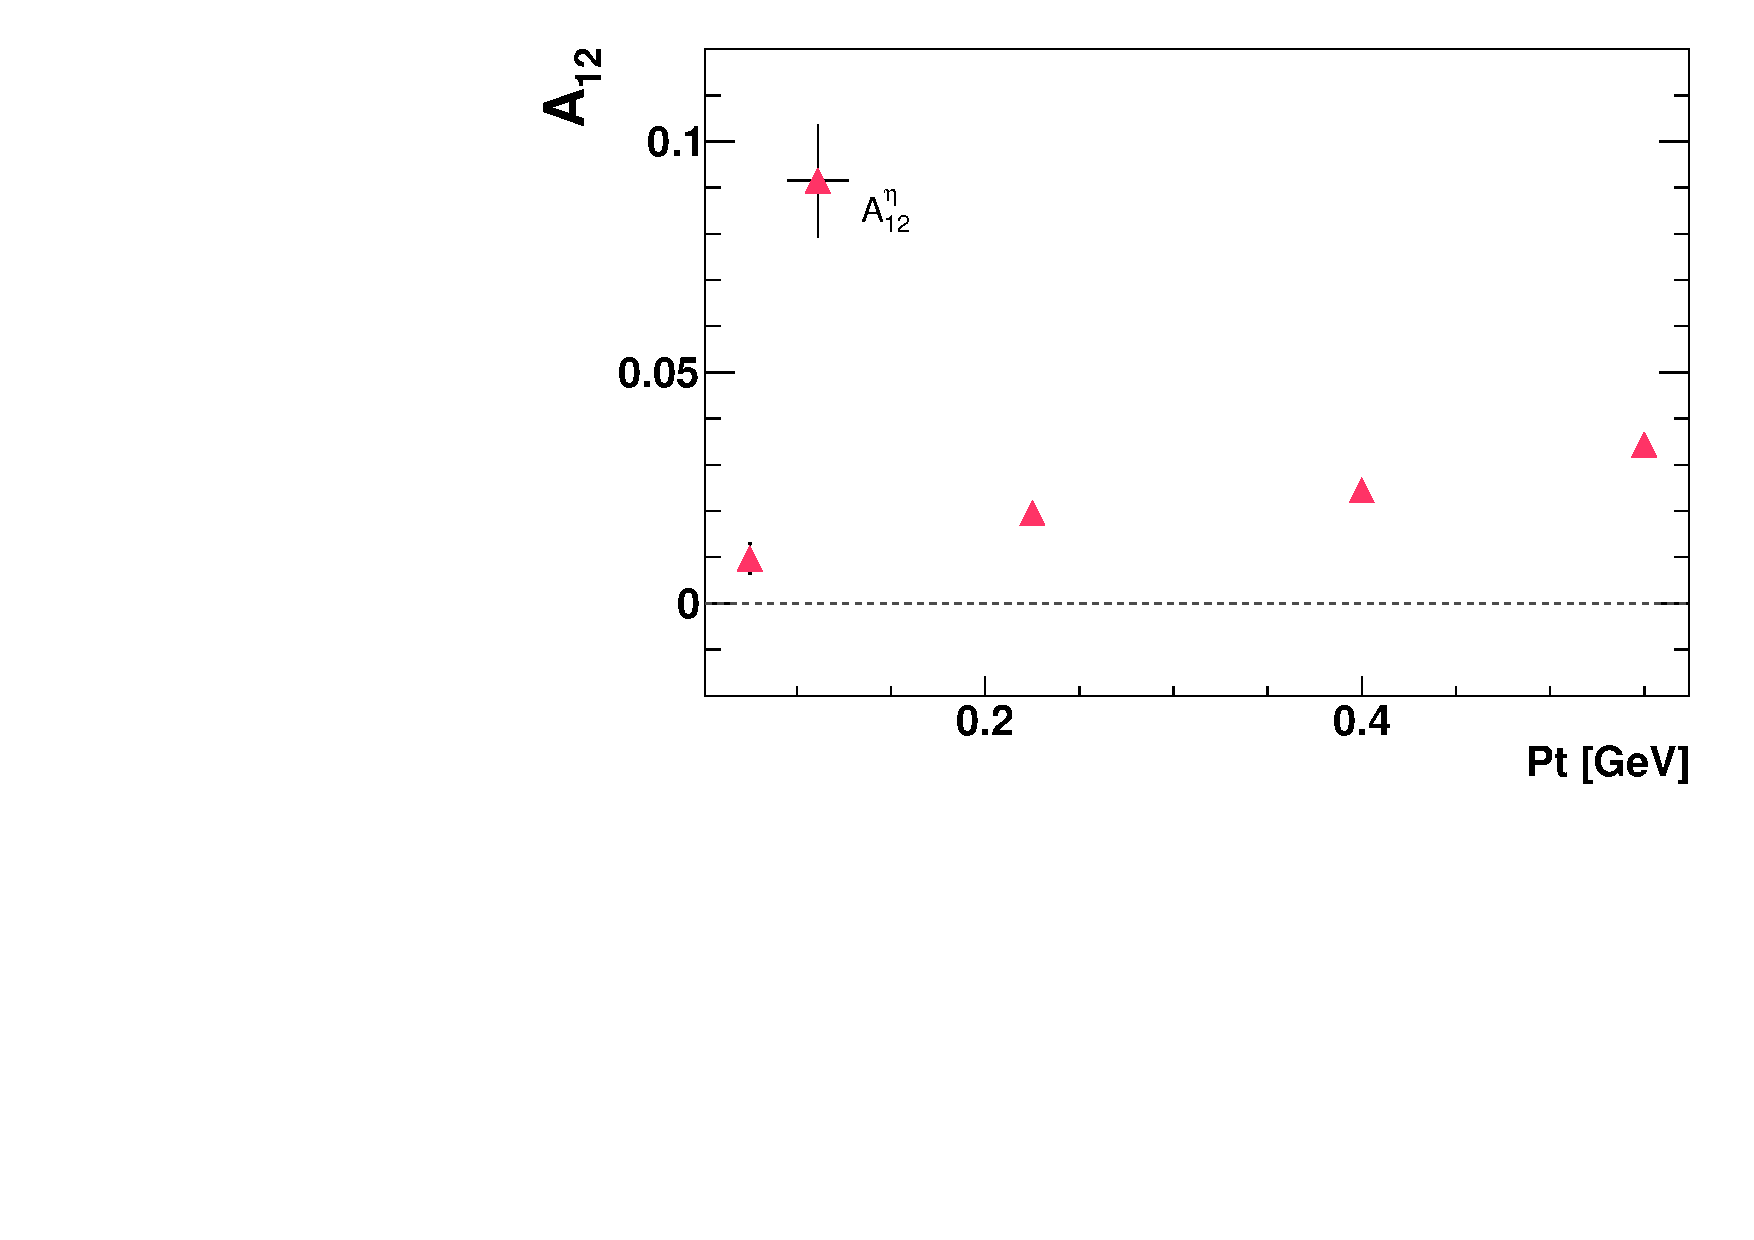
\includegraphics[width=.48\textwidth,natwidth=600,natheight=400]{figure_asy/EtaNoCorrection2.pdf}}
  \subfigure[$\eta$ $(z_1,z_2)$ bins asymmetry]{\label{fig:exp_singlept_eta}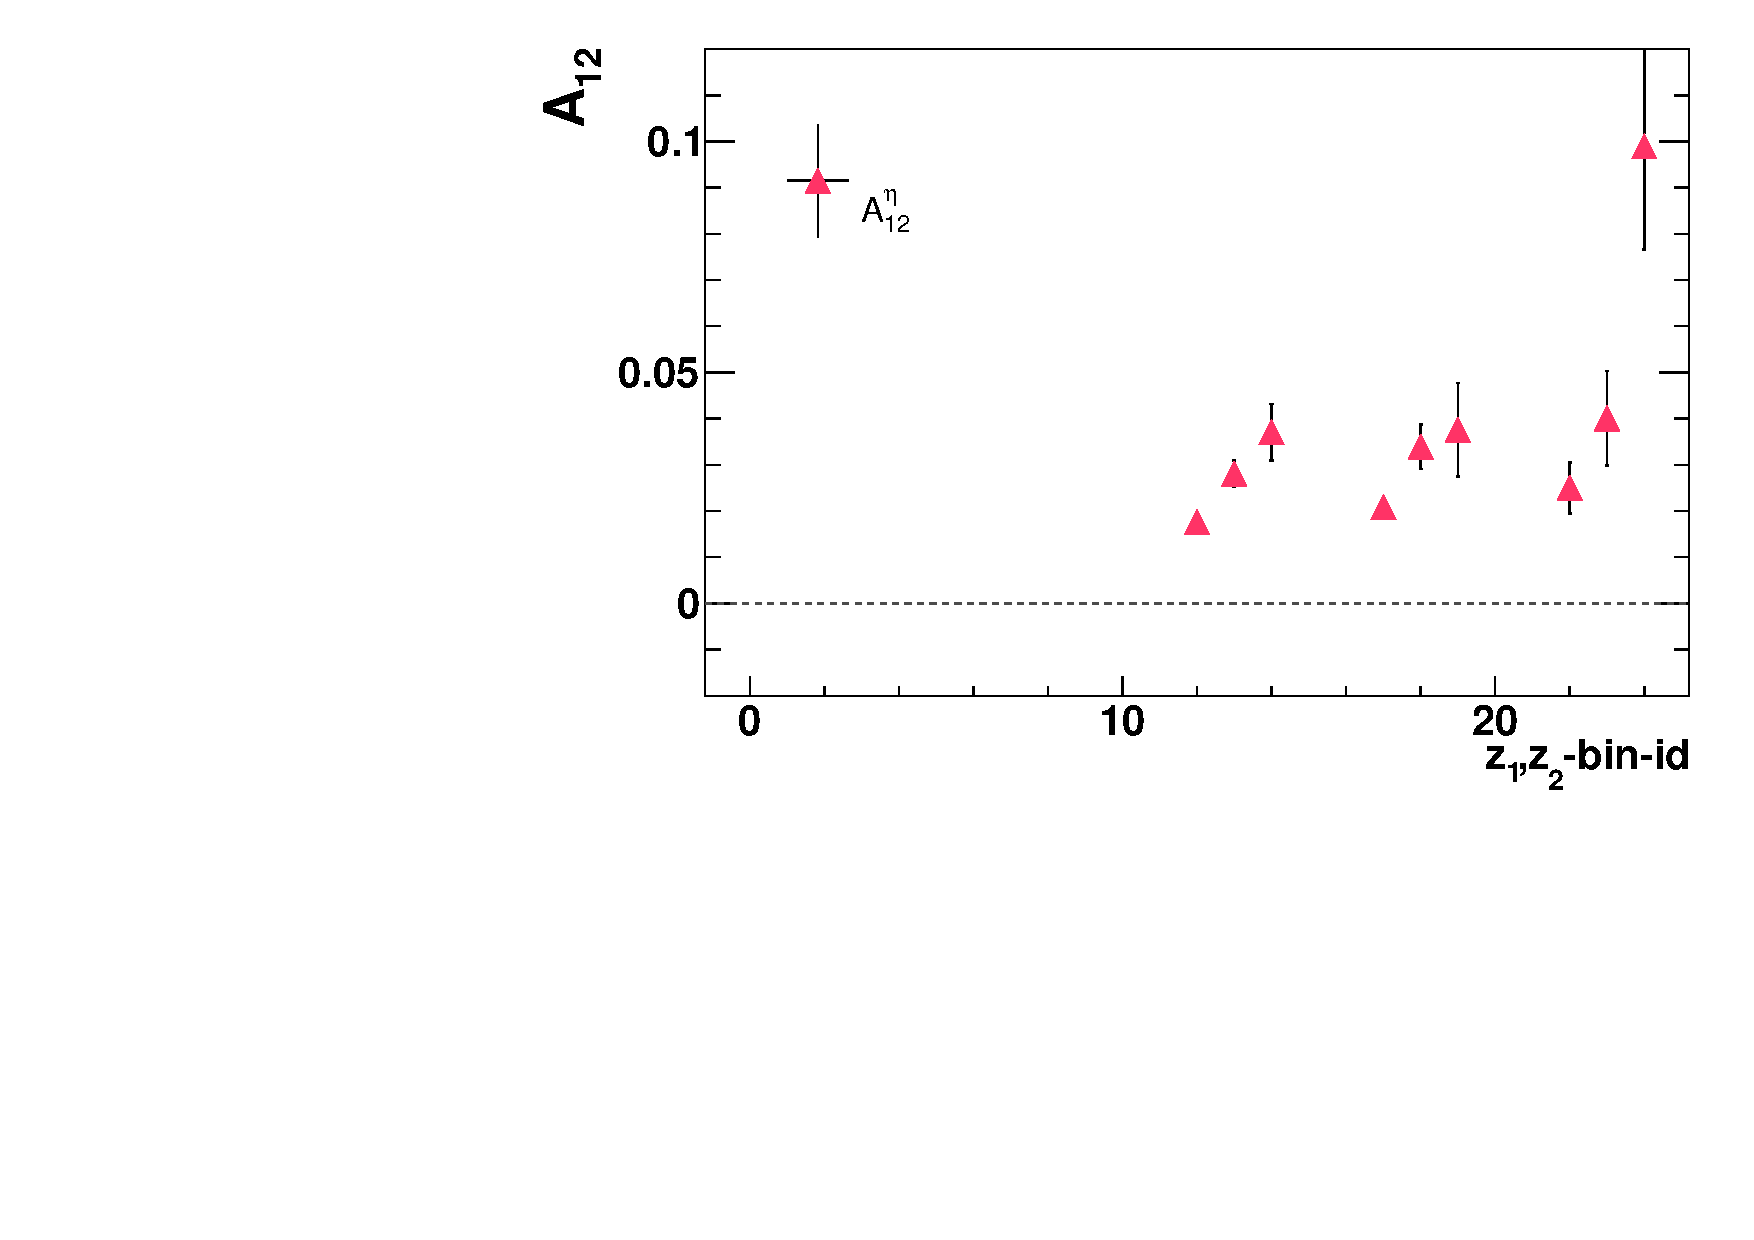
\includegraphics[width=.48\textwidth,natwidth=600,natheight=400]{figure_asy/EtaNoCorrection1.pdf}}
  \subfigure[$\eta$ $(P_{t1},P_{t2})$ bins asymmetry]{\label{fig:exp_compt1_eta}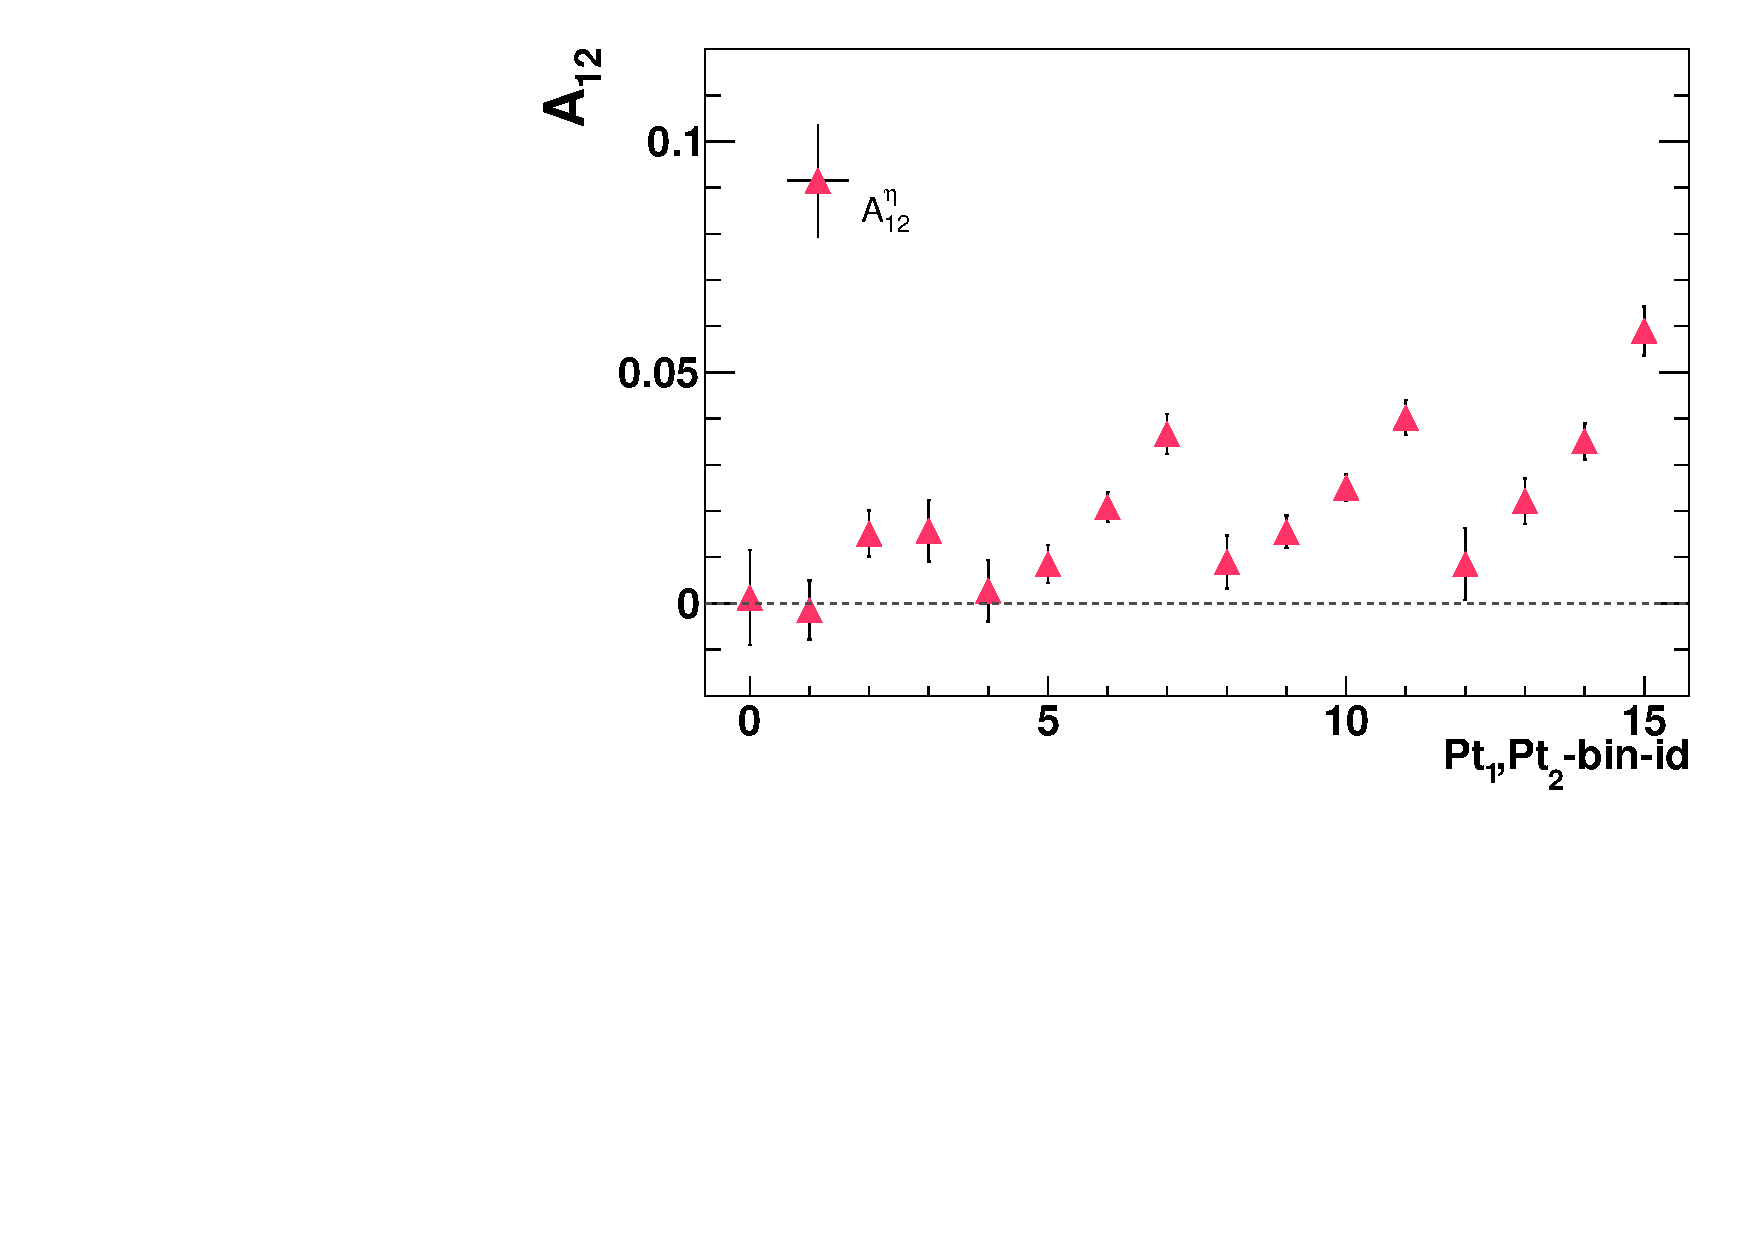
\includegraphics[width=.48\textwidth,natwidth=600,natheight=400]{figure_asy/EtaNoCorrection3.pdf}}
  \caption{Experiment $\eta$ double ratio asymmetry $\nicefrac{A^{\eta\pm}_1}{A^L_1}$}
  \label{fig:exp_eta_result}
\end{figure}

\subsubsection{\texorpdfstring{Other Raw Asymmetries}{Other Raw asymmetries}}
To compare the asymmetry of $\eta$ and $\pi^0$ the $z$ energy threshold $0.3$ is applied on all hadrons contained in $\pi^0$ double ratio. Fig.~\ref{fig:exp_pi0_eta_result} displays  the comparison between $\pi^0$ and $\eta$ for the fractional-energy constraint of $z>0.3$. 

\begin{figure}[H]
  \centering     
  \subfigure[$\pi^0$ and $\eta$ $z_1$ bins asymmetry]{\label{fig:exp_singlez_compare}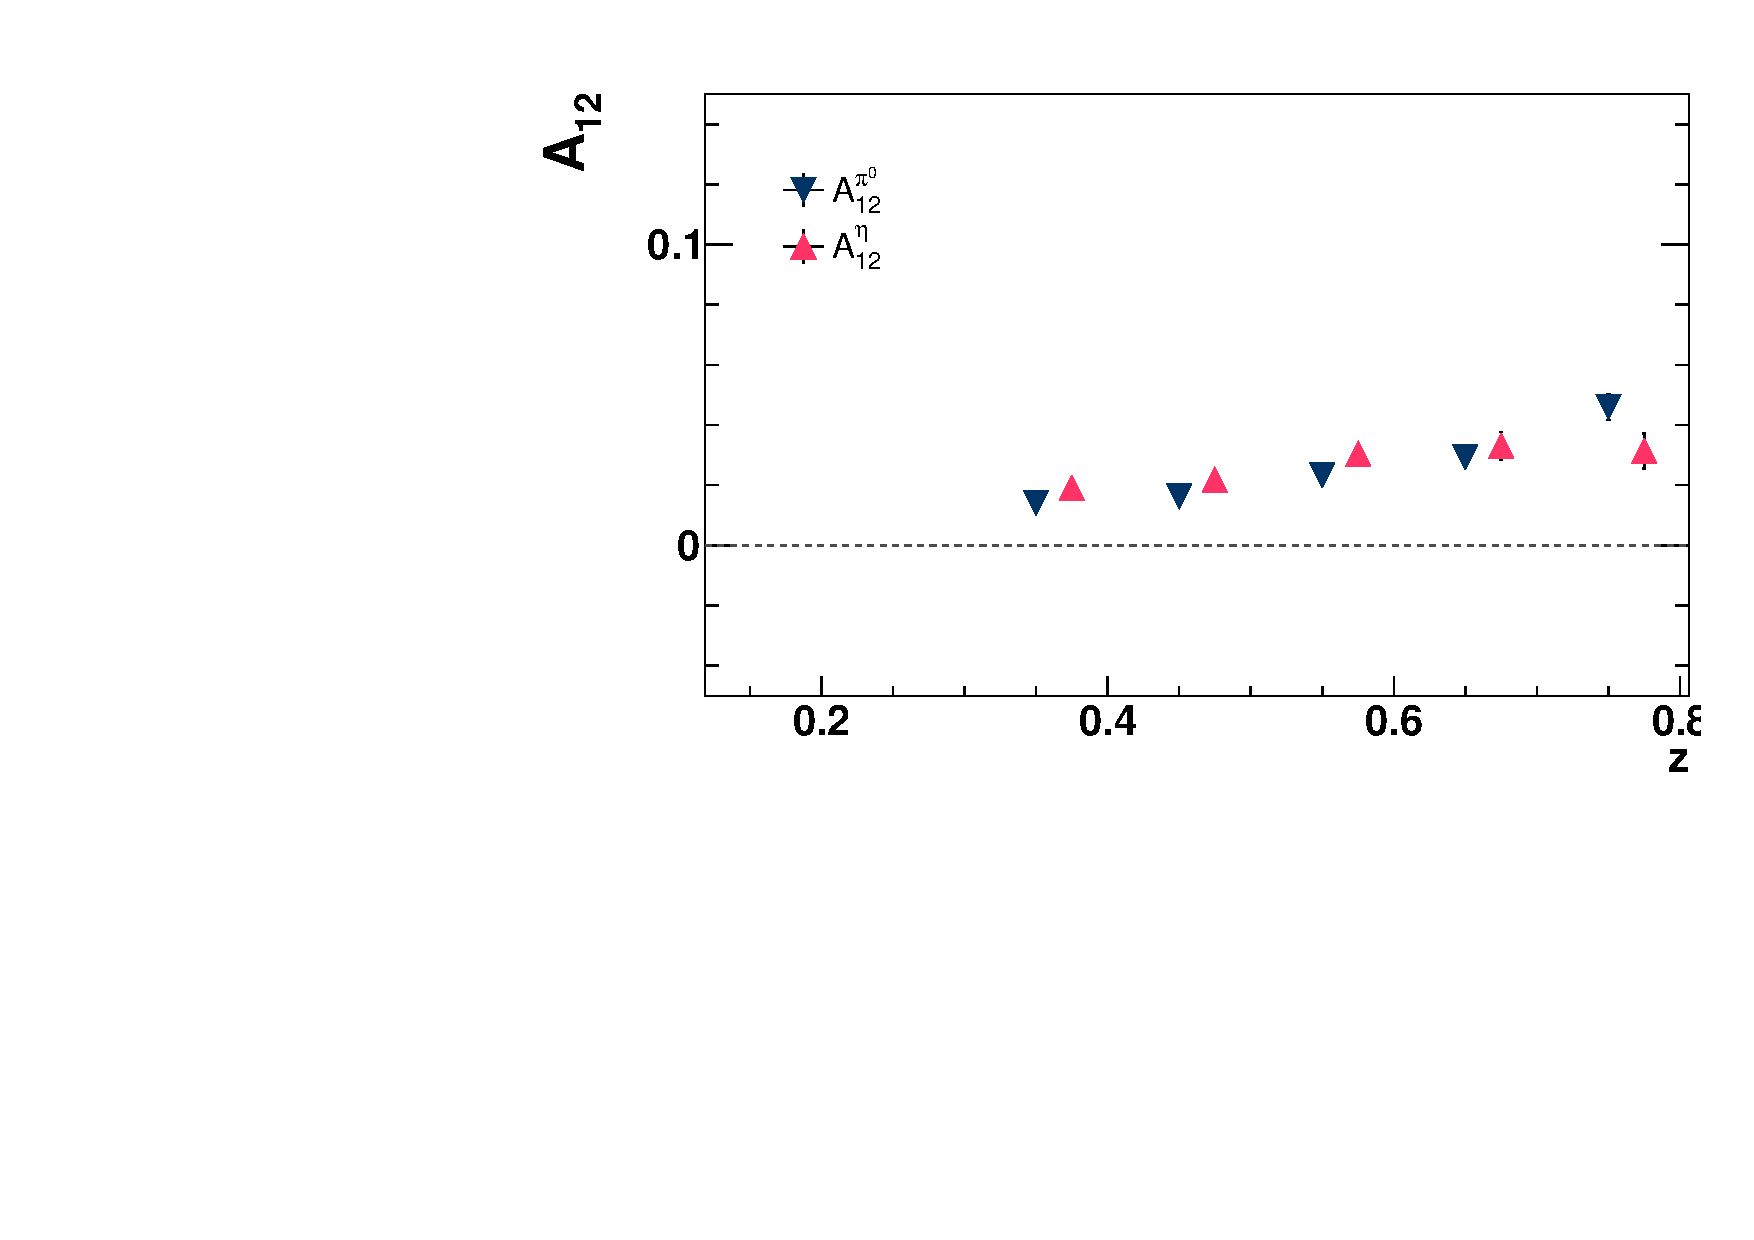
\includegraphics[width=.48\textwidth,natwidth=600,natheight=400]{figure_asy/Pi0VsEta0.pdf}}
  \subfigure[$\pi^0$ and $\eta$ $P_{t1}$ bins asymmetry]{\label{fig:exp_comz_compare}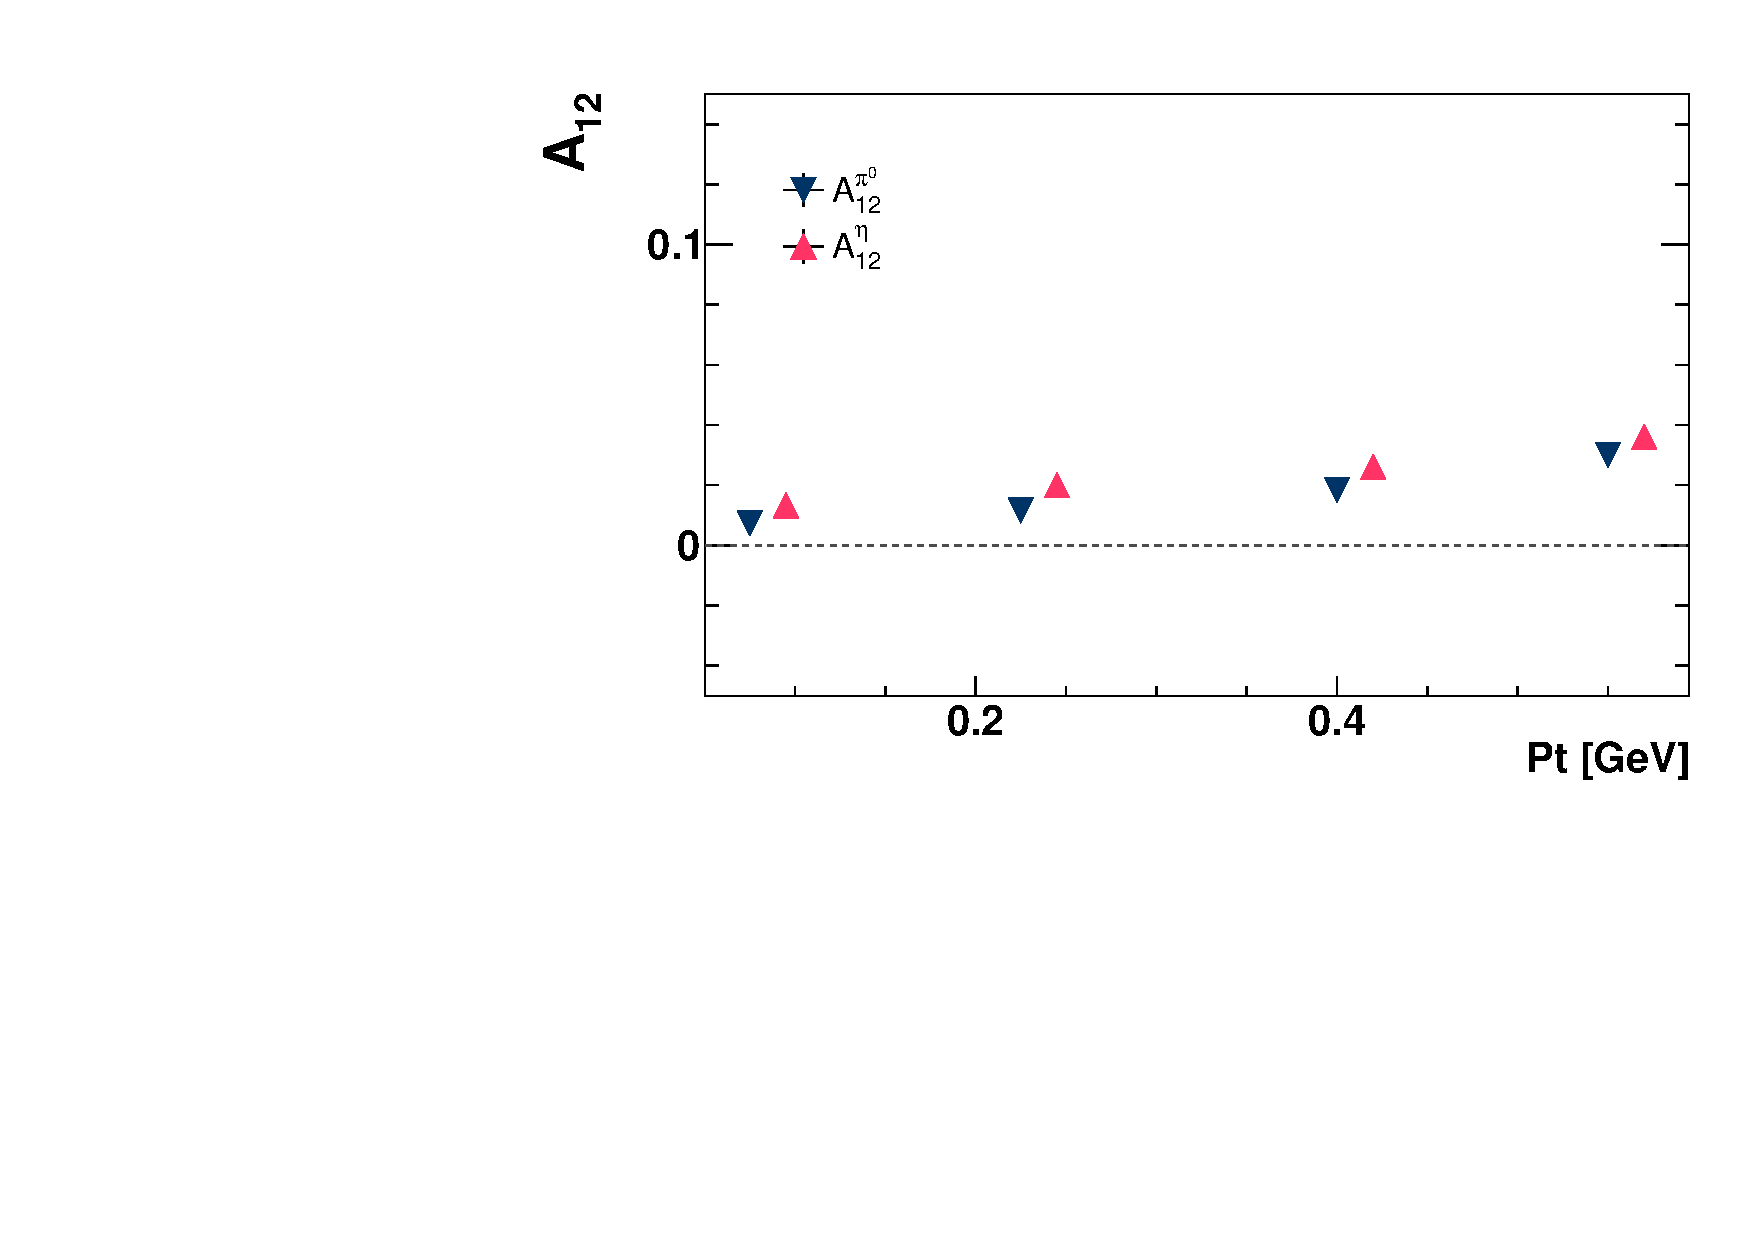
\includegraphics[width=.48\textwidth,natwidth=600,natheight=400]{figure_asy/Pi0VsEta2.pdf}}
  \subfigure[$\pi^0$ and $\eta$ $(z_1,z_2)$ bins asymmetry]{\label{fig:exp_singlept_compare}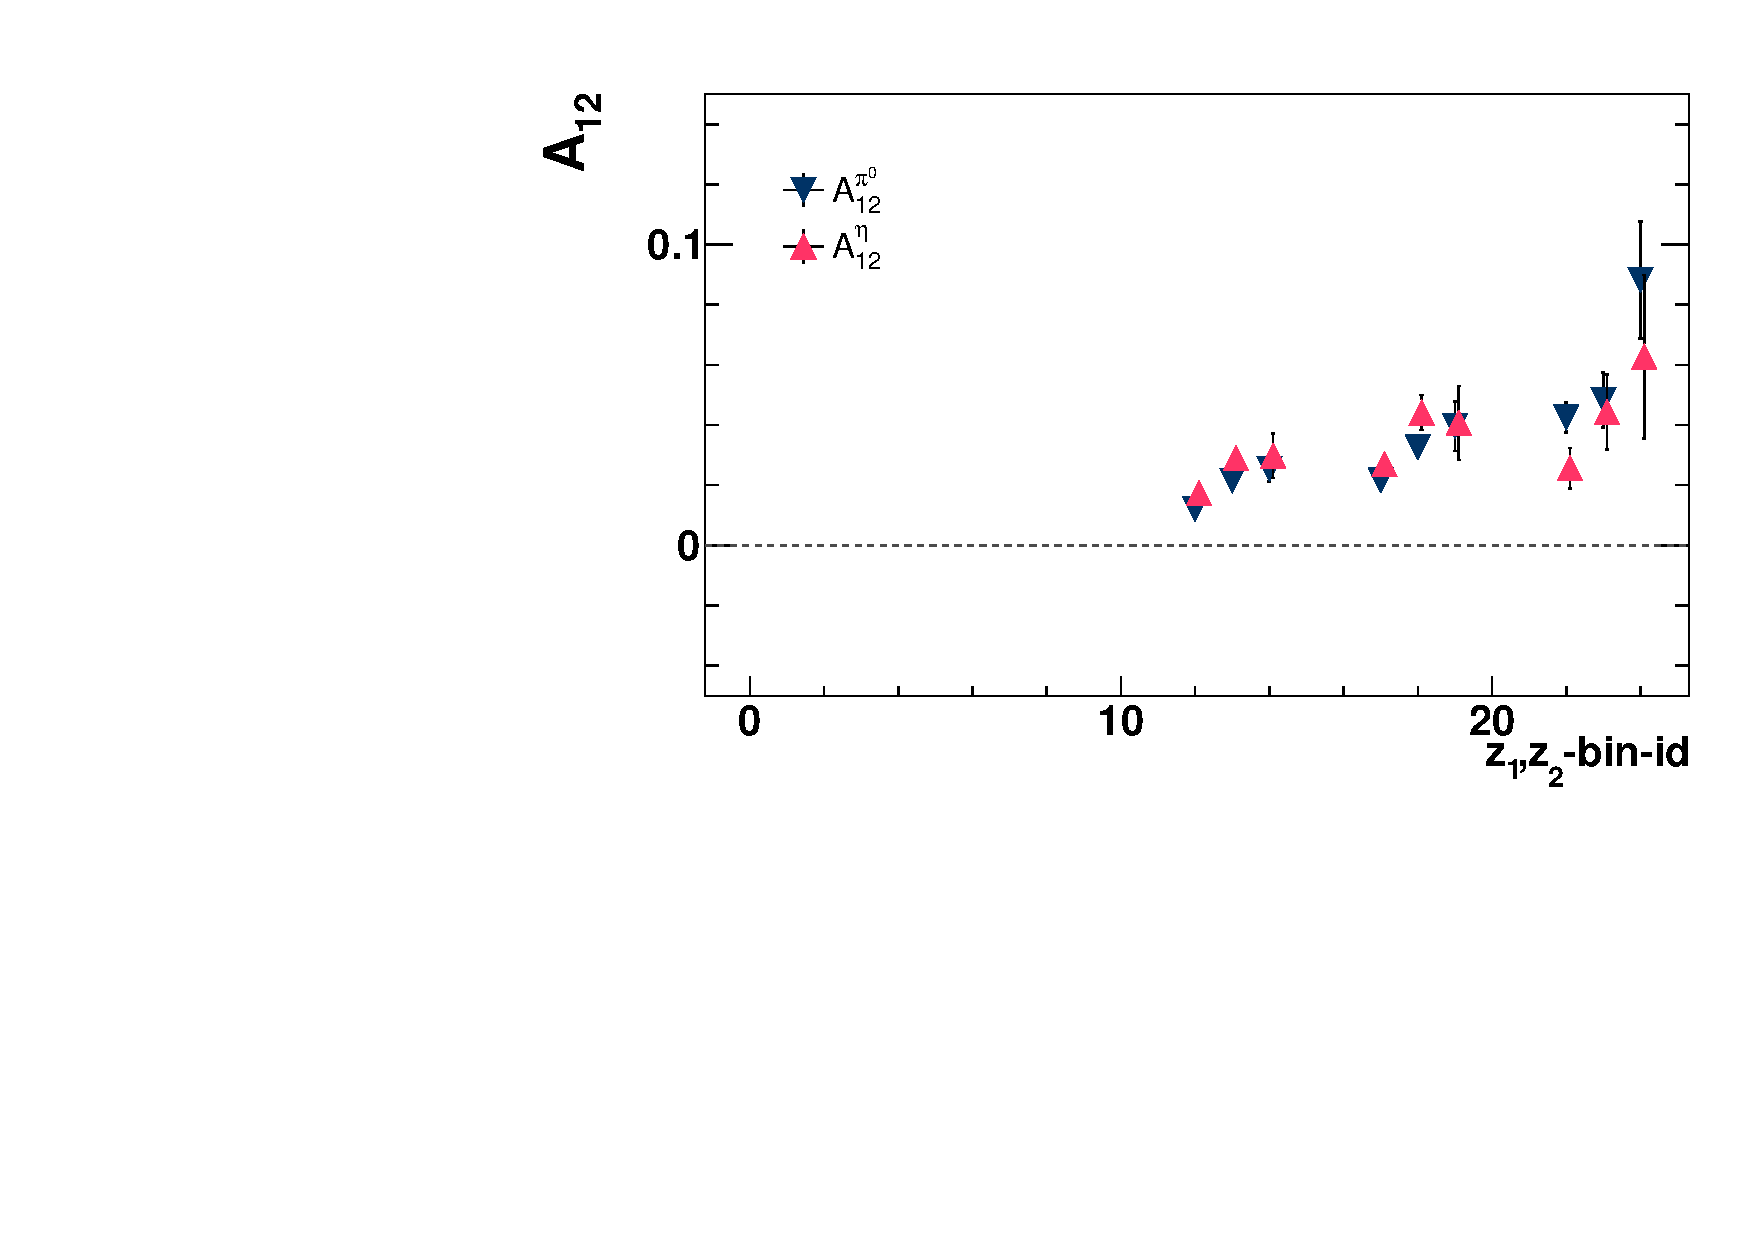
\includegraphics[width=.48\textwidth,natwidth=600,natheight=400]{figure_asy/Pi0VsEta1.pdf}}
  \subfigure[$\pi^0$ and $\eta$ $(P_{t1},P_{t2})$ bins asymmetry]{\label{fig:exp_compt_compare}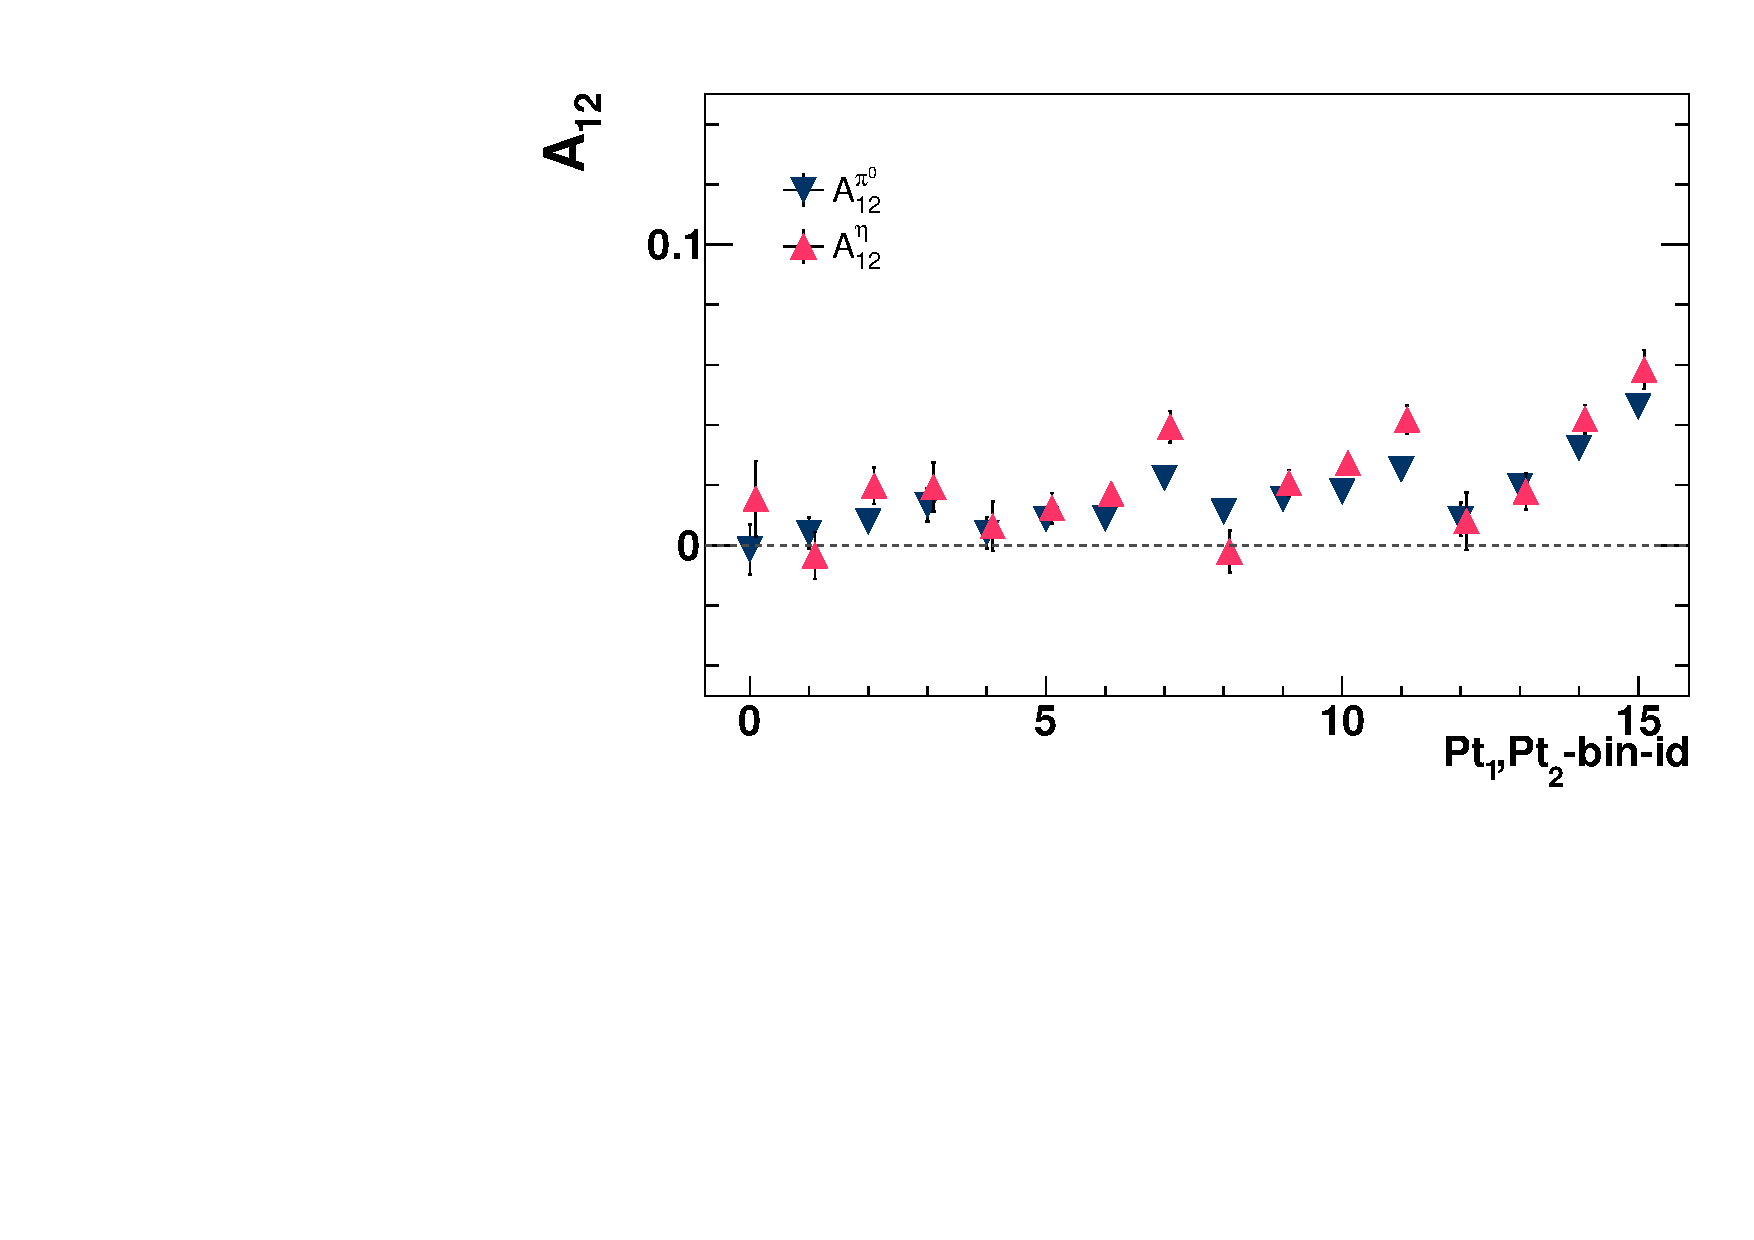
\includegraphics[width=.48\textwidth,natwidth=600,natheight=400]{figure_asy/Pi0VsEta3.pdf}}
  \caption{$\pi^0$ double ratio asymmetry $\nicefrac{A^{0\pm}_{12}}{A^L_{12}}$ and $\eta$ double ratio asymmetry $\nicefrac{A^{\eta\pm}_{12}}{A^L_{12}}$. The down pointing triangles are $\eta$ asymmetries and up pointing triangles are $\pi^0$ asymmetries.}
  \label{fig:exp_pi0_eta_result}
\end{figure}
The following plots show the ratio between $\pi^0$ and $\eta$ asymmetries. Besides the uncertainty caused by statistics, $\pi^0$ shows different asymmetries than $\eta$ at some bins. This could be caused by, eg., the expected difference in the fragmentation of strange quarks or by differences between detection efficiencies of $\pi^0$ and $\eta$. However, this difference is nonsignificant at this stage and more precise conclusion will be discussed after the correction of thrust smearing effect.
\begin{figure}[H]
  \centering     
  \subfigure[$\pi^0$ over $\eta$ double ratio $z_1$ bins]{\label{fig:exp_singlez_ratio}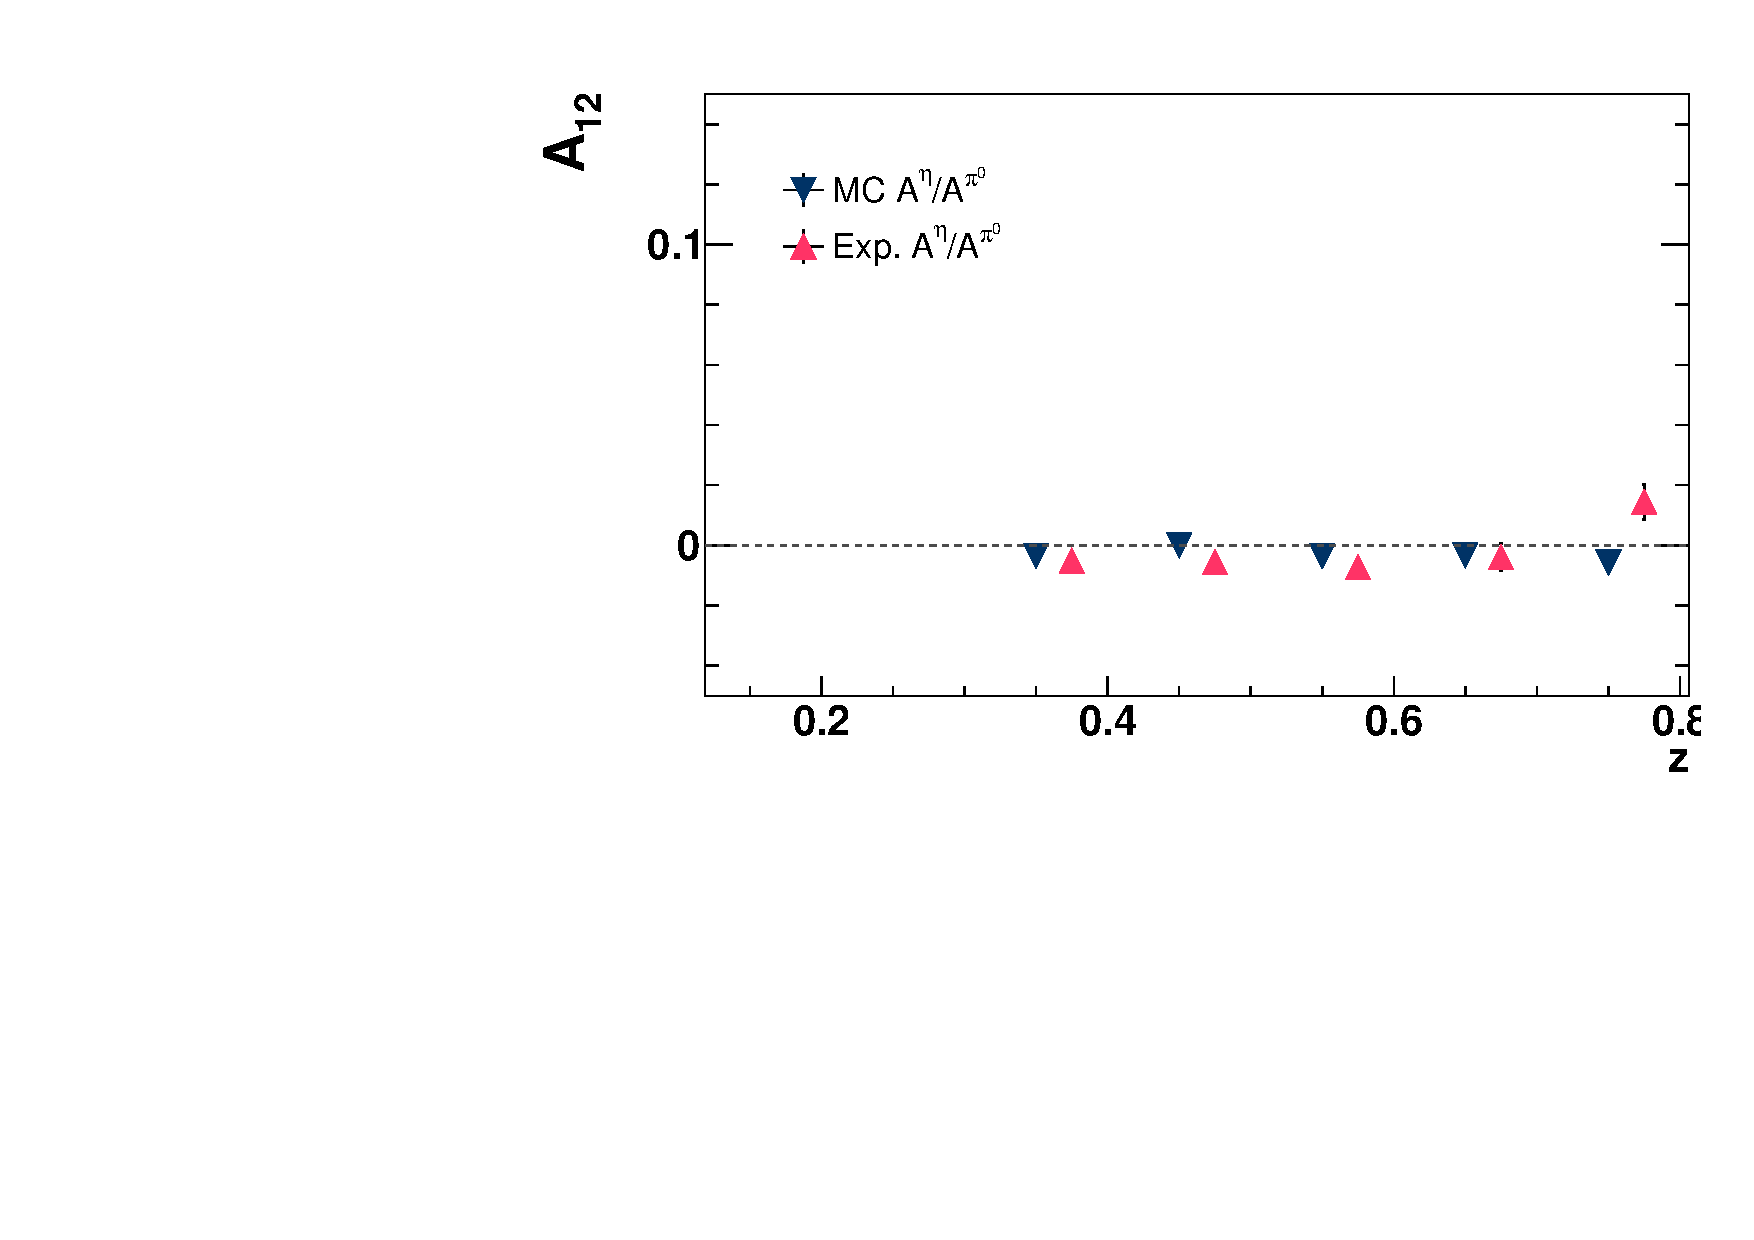
\includegraphics[width=.48\textwidth,natwidth=600,natheight=400]{figure_asy/Pi0OverEta0.pdf}}
   \subfigure[$\pi^0$ over $\eta$ double ratio $P_{t1}$ bins]{\label{fig:exp_comz_ratio}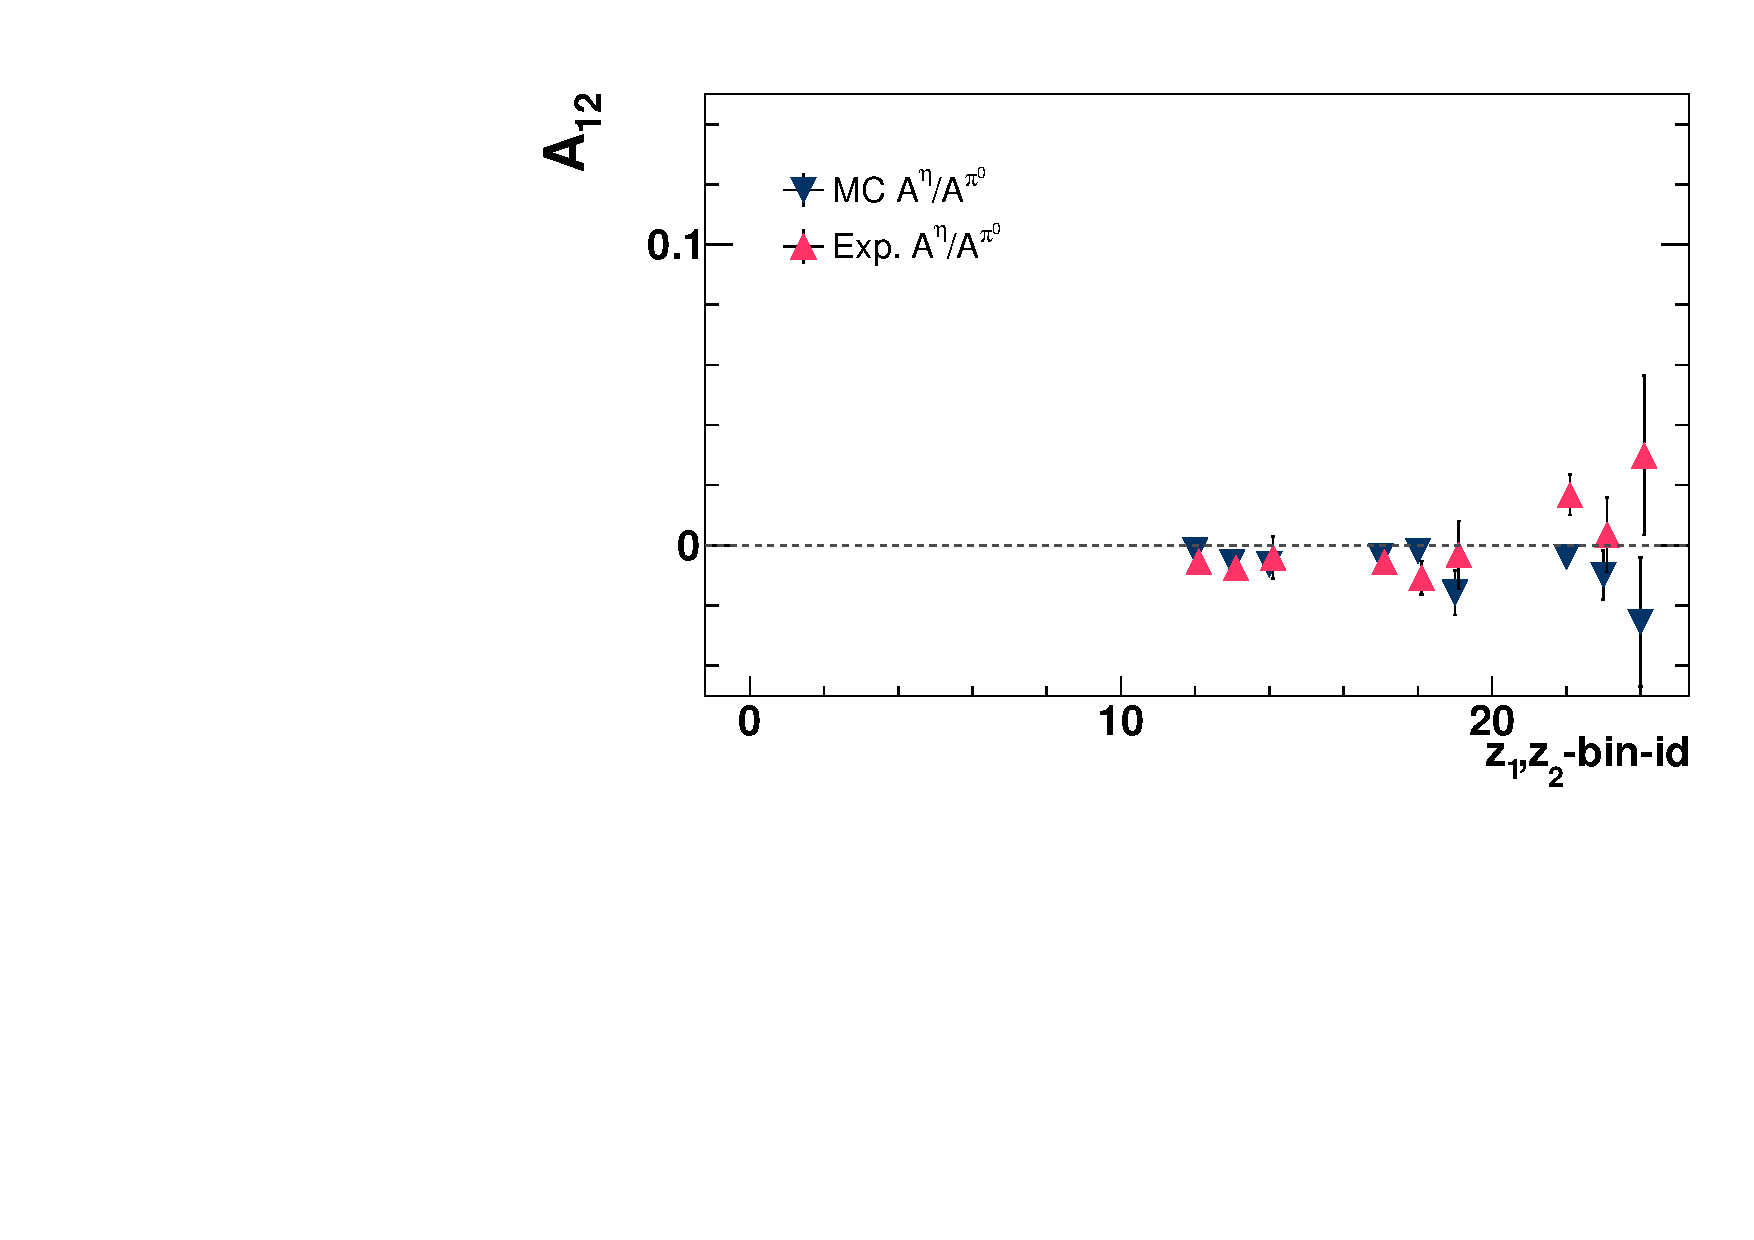
\includegraphics[width=.48\textwidth,natwidth=600,natheight=400]{figure_asy/Pi0OverEta1.pdf}}
  \subfigure[$\pi^0$ over $\eta$ double ratio $(z_1,z_2)$ bins]{\label{fig:exp_signlept_ratio}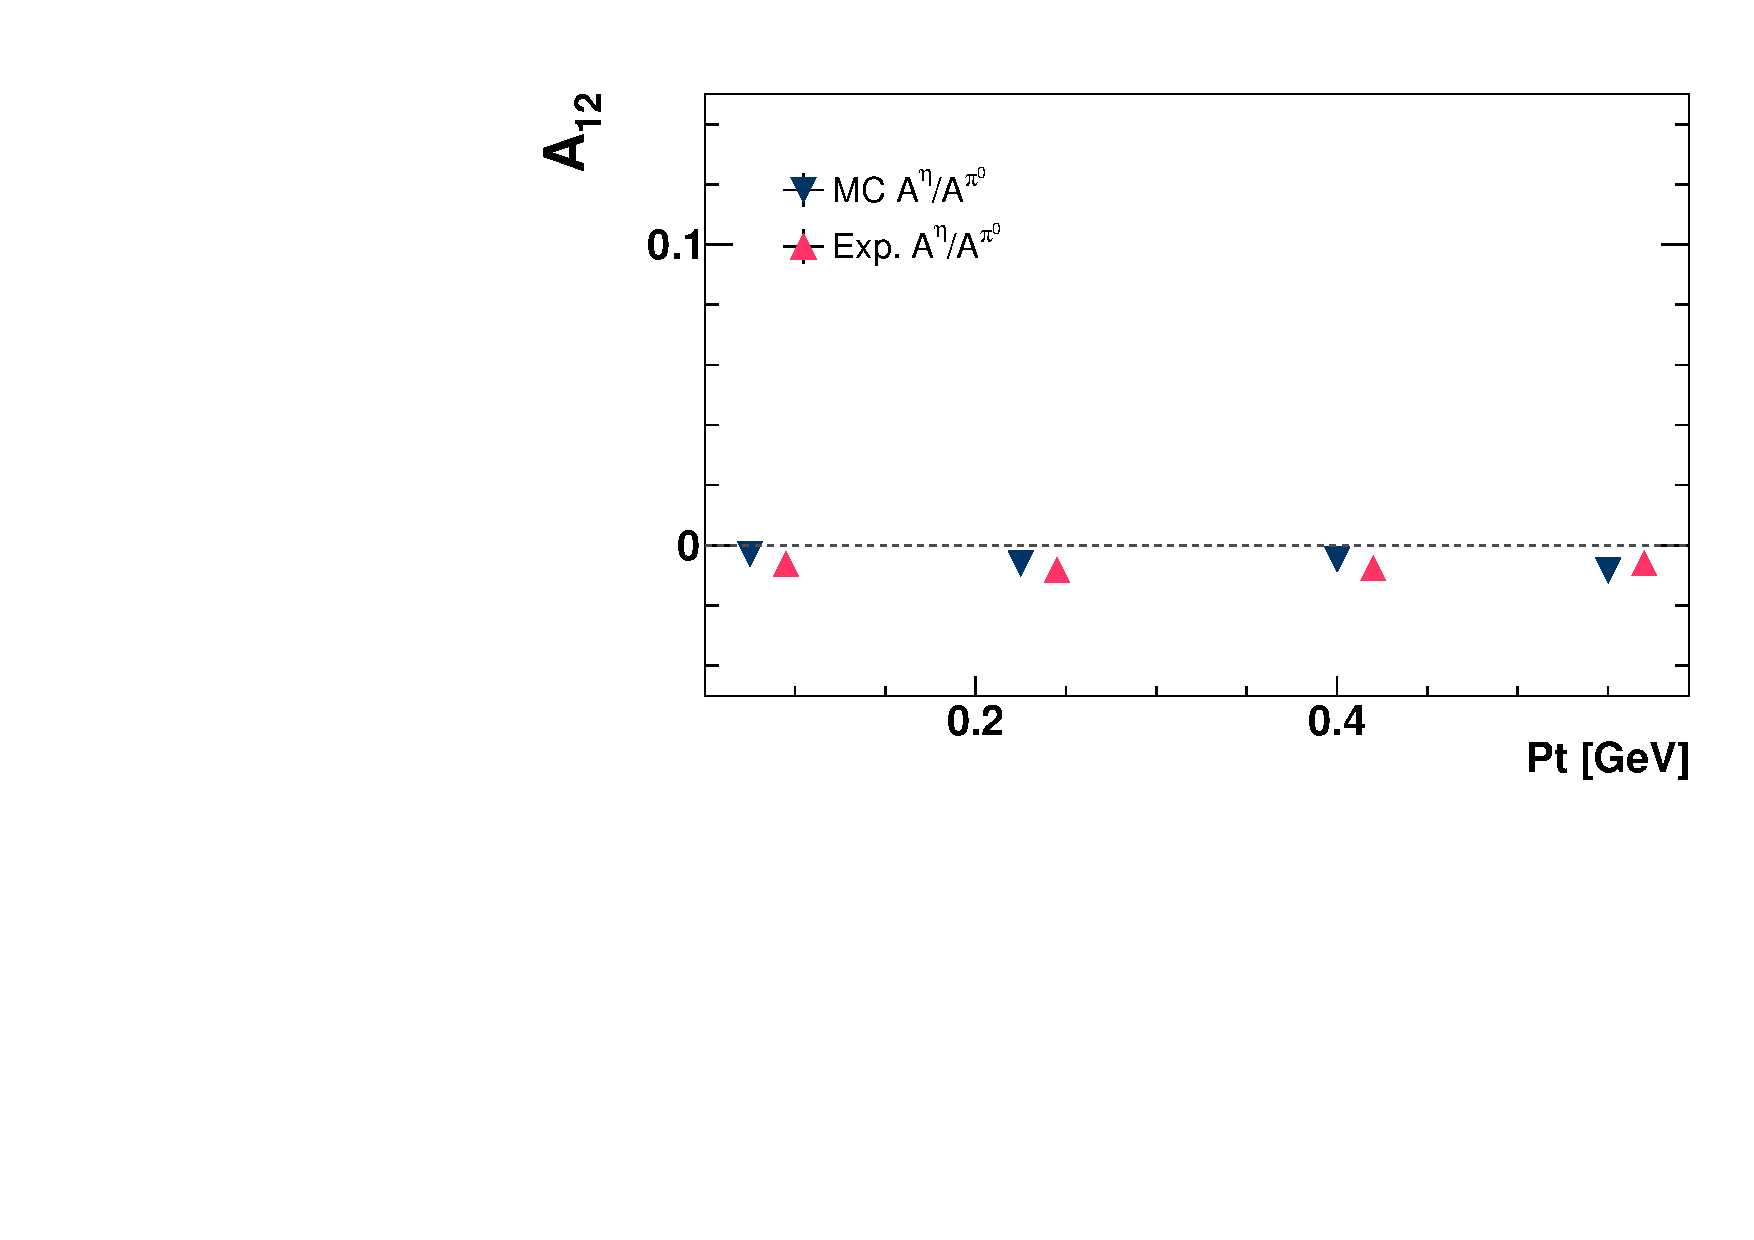
\includegraphics[width=.48\textwidth,natwidth=600,natheight=400]{figure_asy/Pi0OverEta2.pdf}}
  \subfigure[$\pi^0$ over $\eta$ double ratio $(P_{t1},P_{t2})$ bins]{\label{fig:exp_compt_ratio}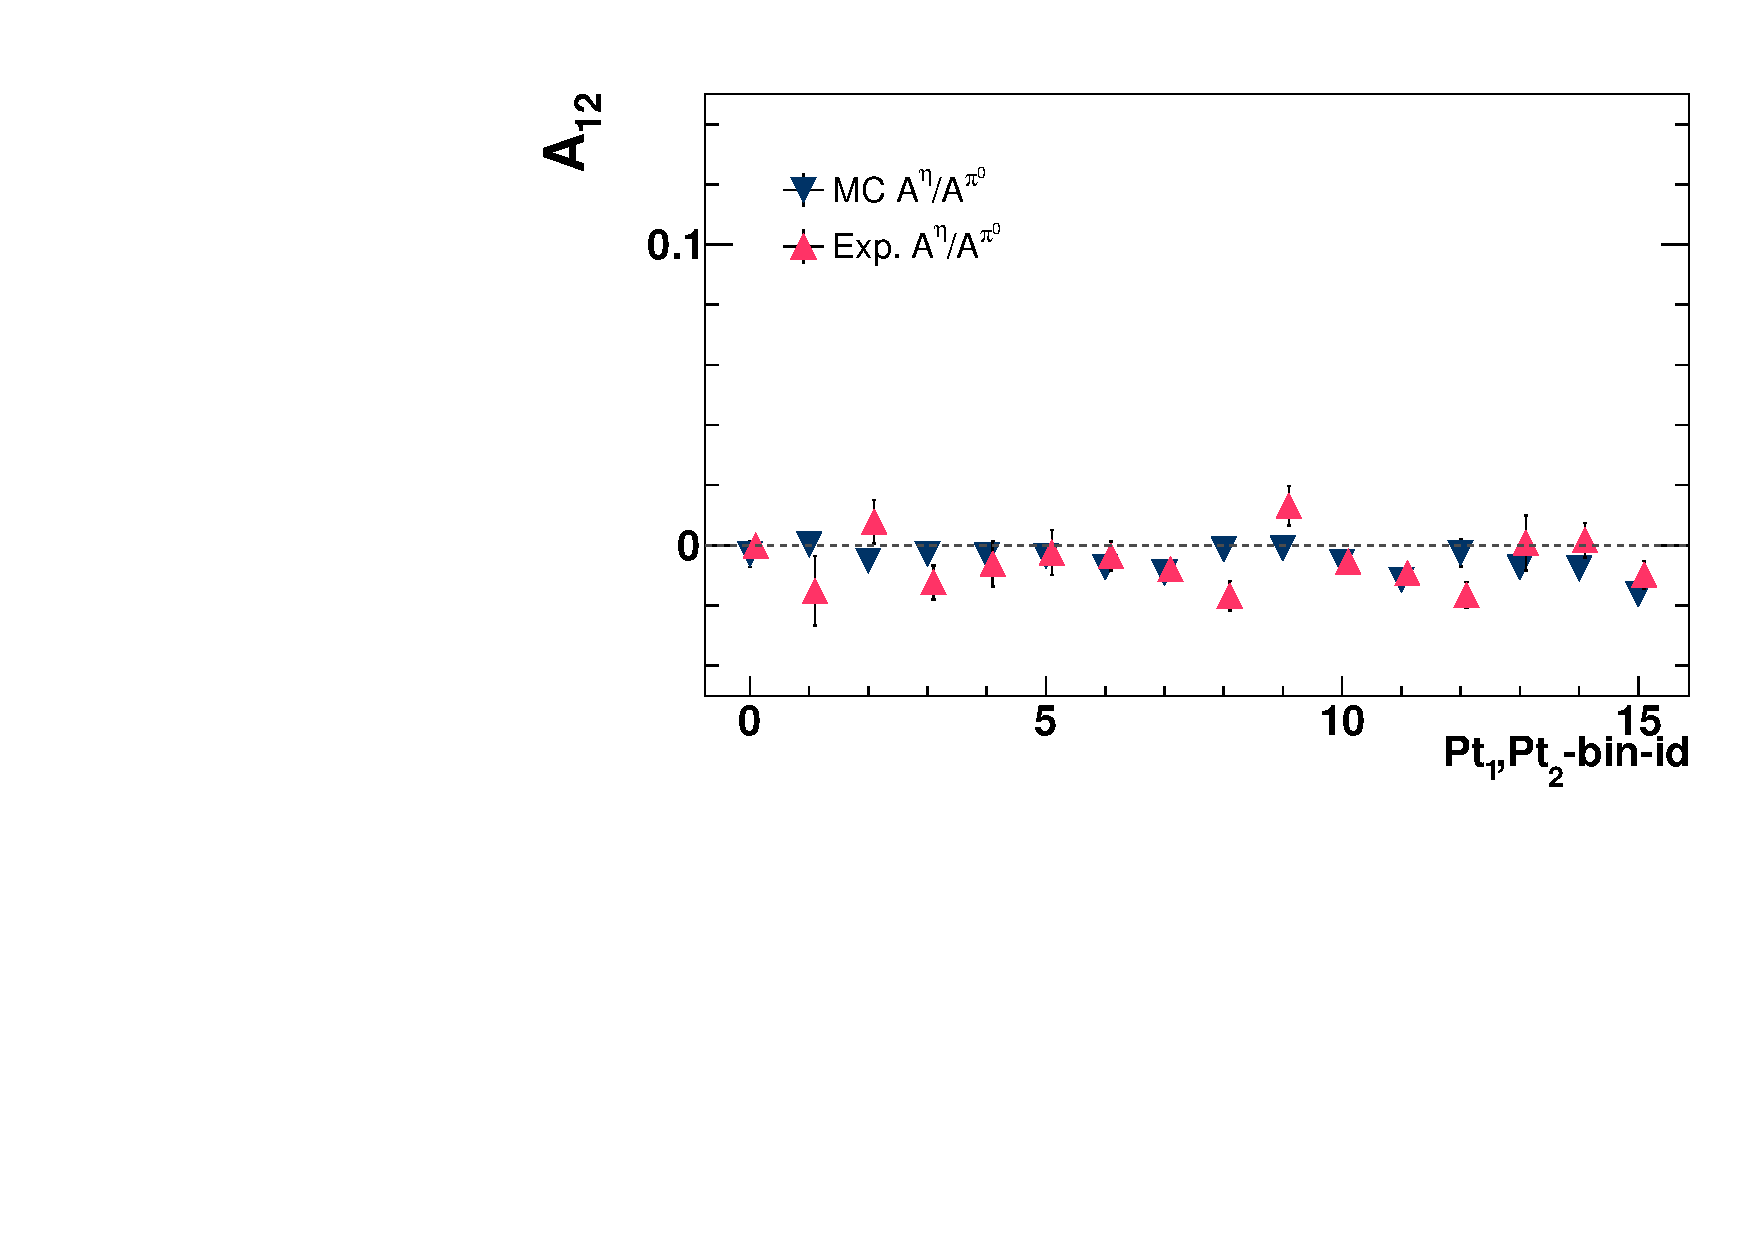
\includegraphics[width=.48\textwidth,natwidth=600,natheight=400]{figure_asy/Pi0OverEta3.pdf}}
  \caption{ Asymmetry $\nicefrac{A^{\eta\pm}_{12}}{A^{0\pm}_{12}}$.}
  \label{fig:exp_pi0_eta_ratio}
\end{figure}
As it will be discussed in section~\ref{sec:comparewpreviouse}, the expression of UC double ratio written in Eqn.~\ref{eqn:allratiosexpress} is comparable with $\pi^0$ double ratio~\ref{eqn:FF5}. Here we introduce a new double ratio:
\begin{equation}
\frac{A^{0\pm}_{12}}{A^C_{12}}=\frac{\pi^0\pi^++\pi^0\pi^-}{\pi^+\pi^++\pi^-\pi^++\pi^+\pi^-+\pi^-\pi^-}\\
\end{equation}
If detector effect is eliminated by fiducial cuts, the asymmetry of this new double ratio should be zero using both MC and experimental data. Figure~\ref{fig:exp_pi0_eta_ratio2}demonstrates our theory and indicate good performing of our fiducial cuts.
\begin{figure}[H]
  \centering     
  \subfigure[$\pi^0$ double ratio over UC double ratio $z_1$ bins]{\label{fig:eta_singlez_ratio2}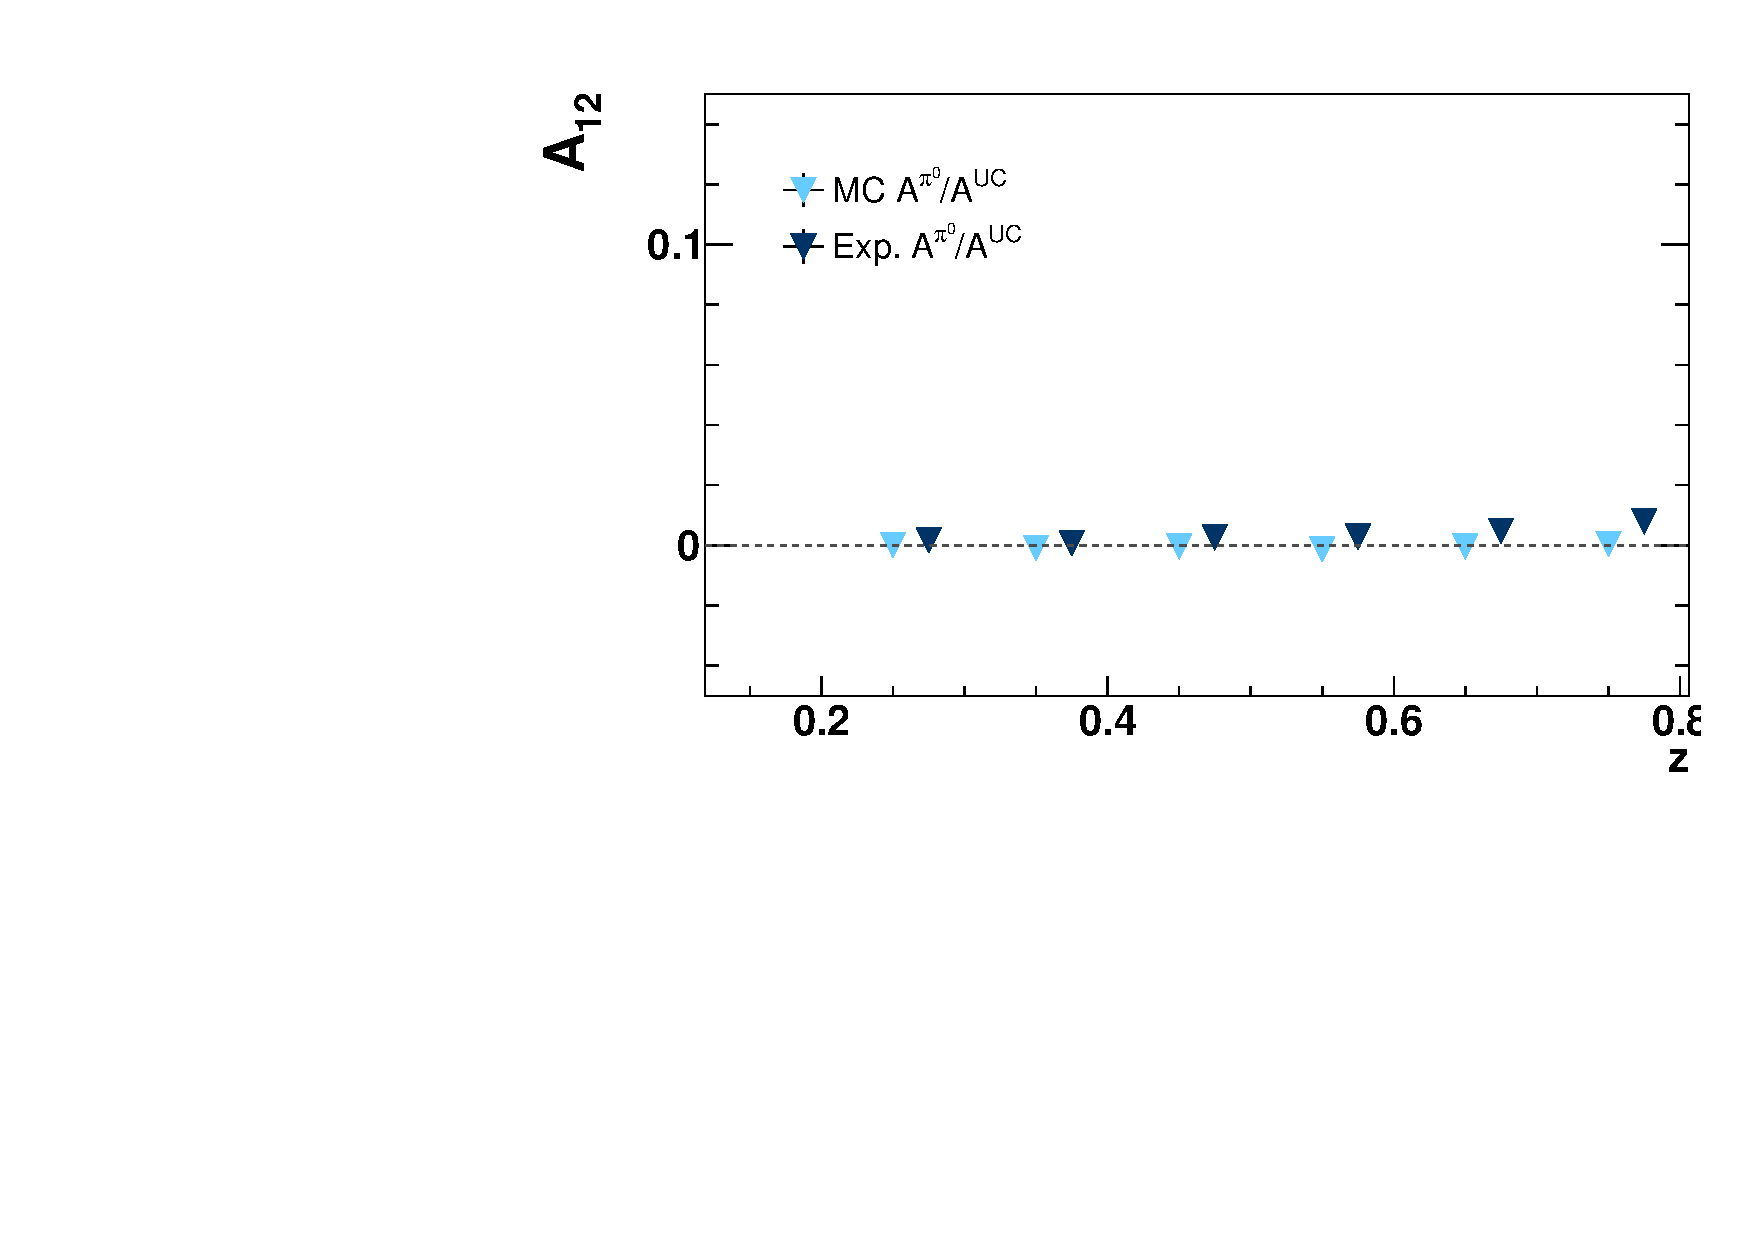
\includegraphics[width=.48\textwidth,natwidth=600,natheight=400]{figure_asy/Pi0OverUC0.pdf}}
   \subfigure[$\pi^0$ double ratio over UC double ratio $P_{t1}$ bins]{\label{fig:exp_comz_ratio2}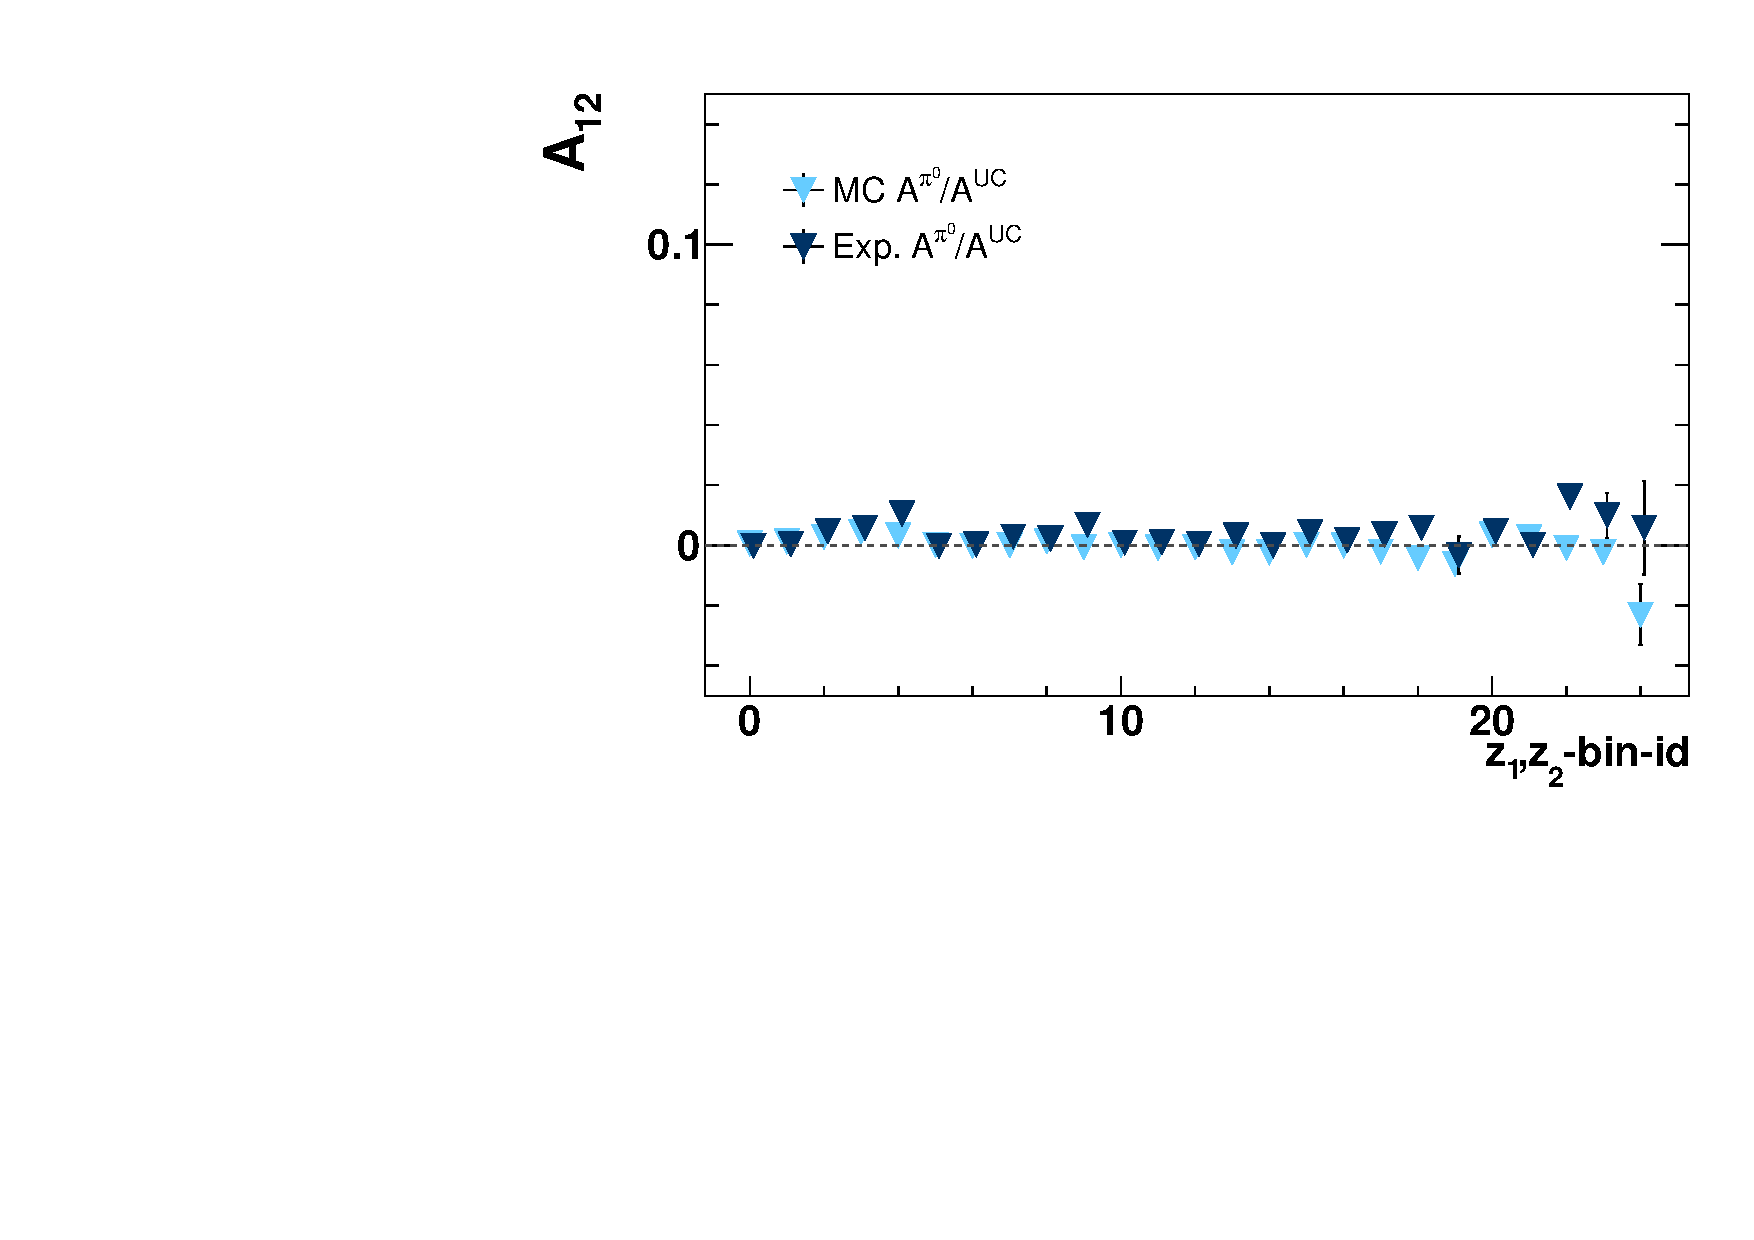
\includegraphics[width=.48\textwidth,natwidth=600,natheight=400]{figure_asy/Pi0OverUC1.pdf}}
  \subfigure[$\pi^0$ double ratio over UC double ratio $(z_1,z_2)$ bins]{\label{fig:exp_signlept_ratio2}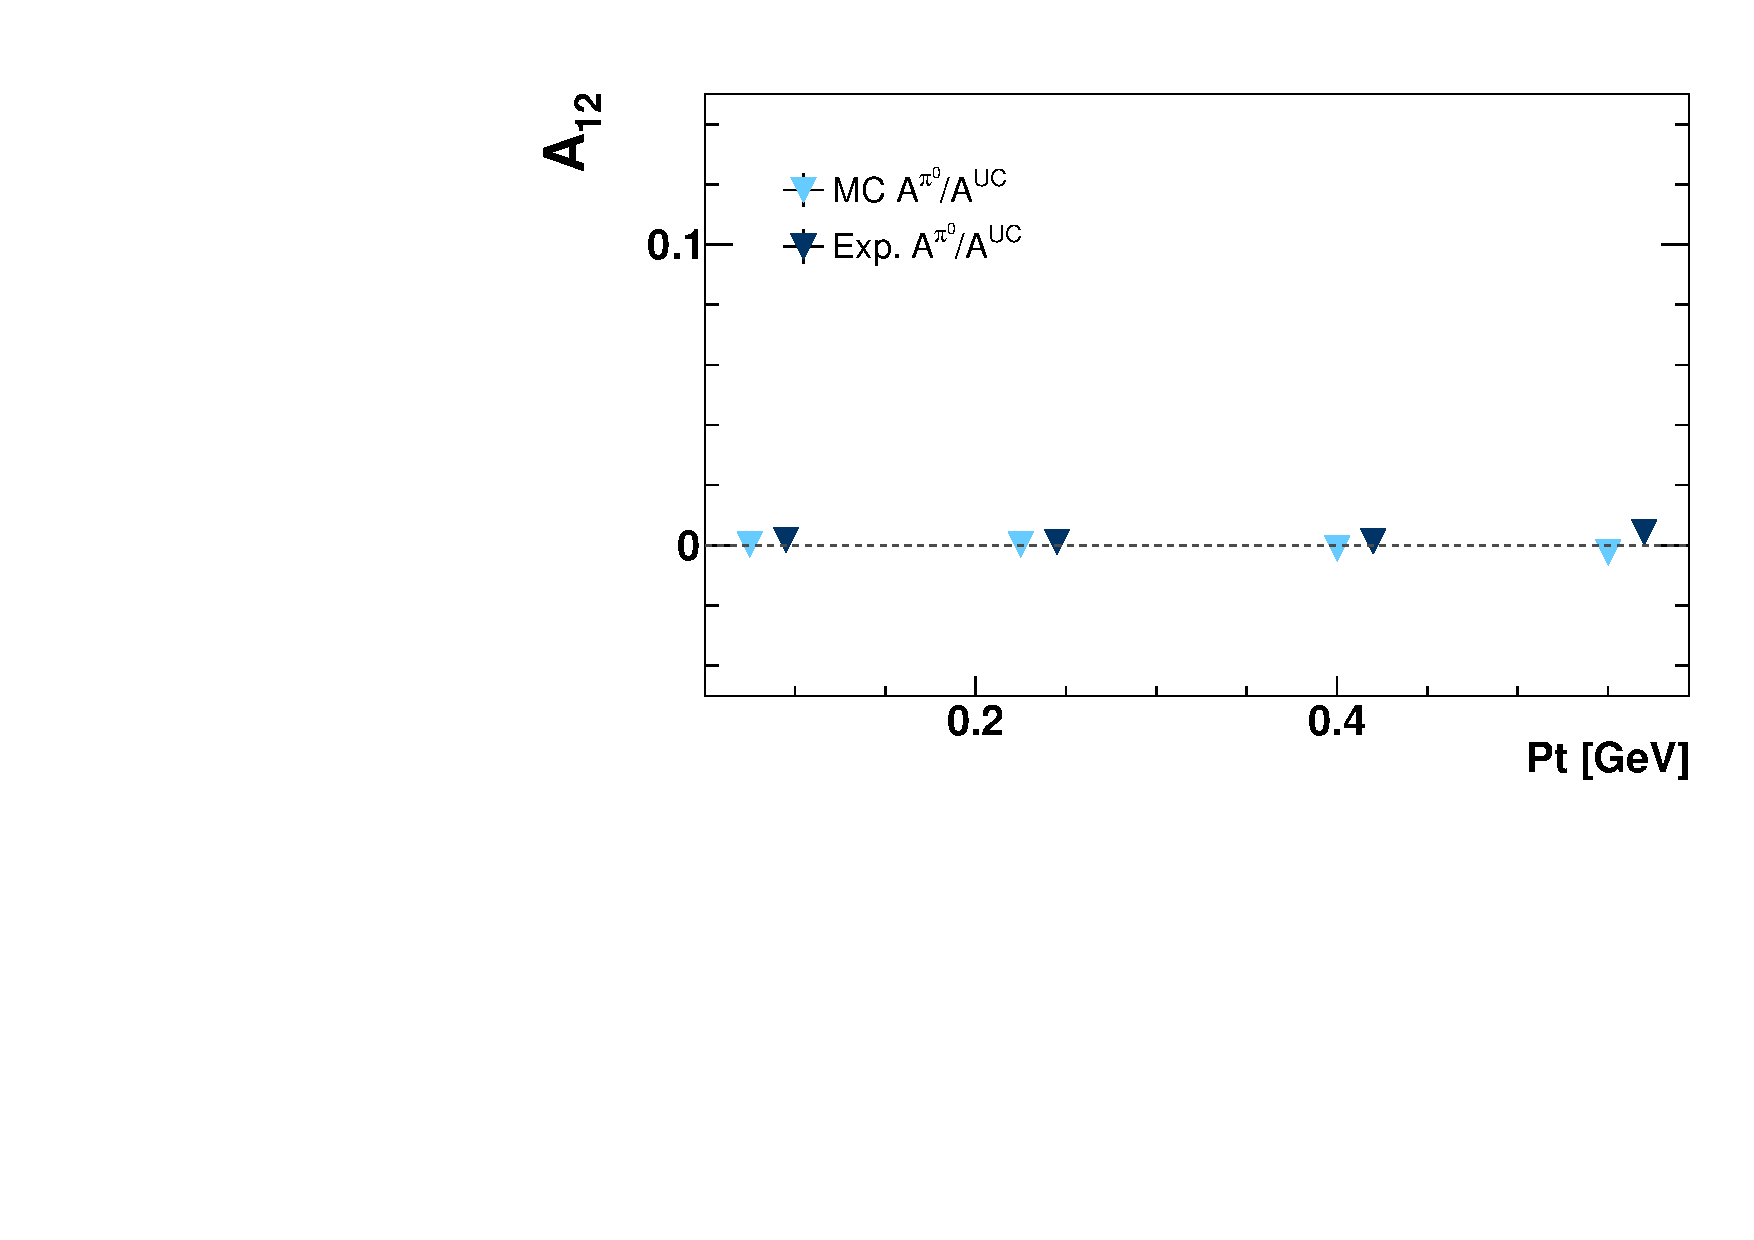
\includegraphics[width=.48\textwidth,natwidth=600,natheight=400]{figure_asy/Pi0OverUC2.pdf}}
  \subfigure[$\pi^0$ double ratio over UC double ratio $(P_{t1},P_{t2})$ bins]{\label{fig:exp_compt_ratio2}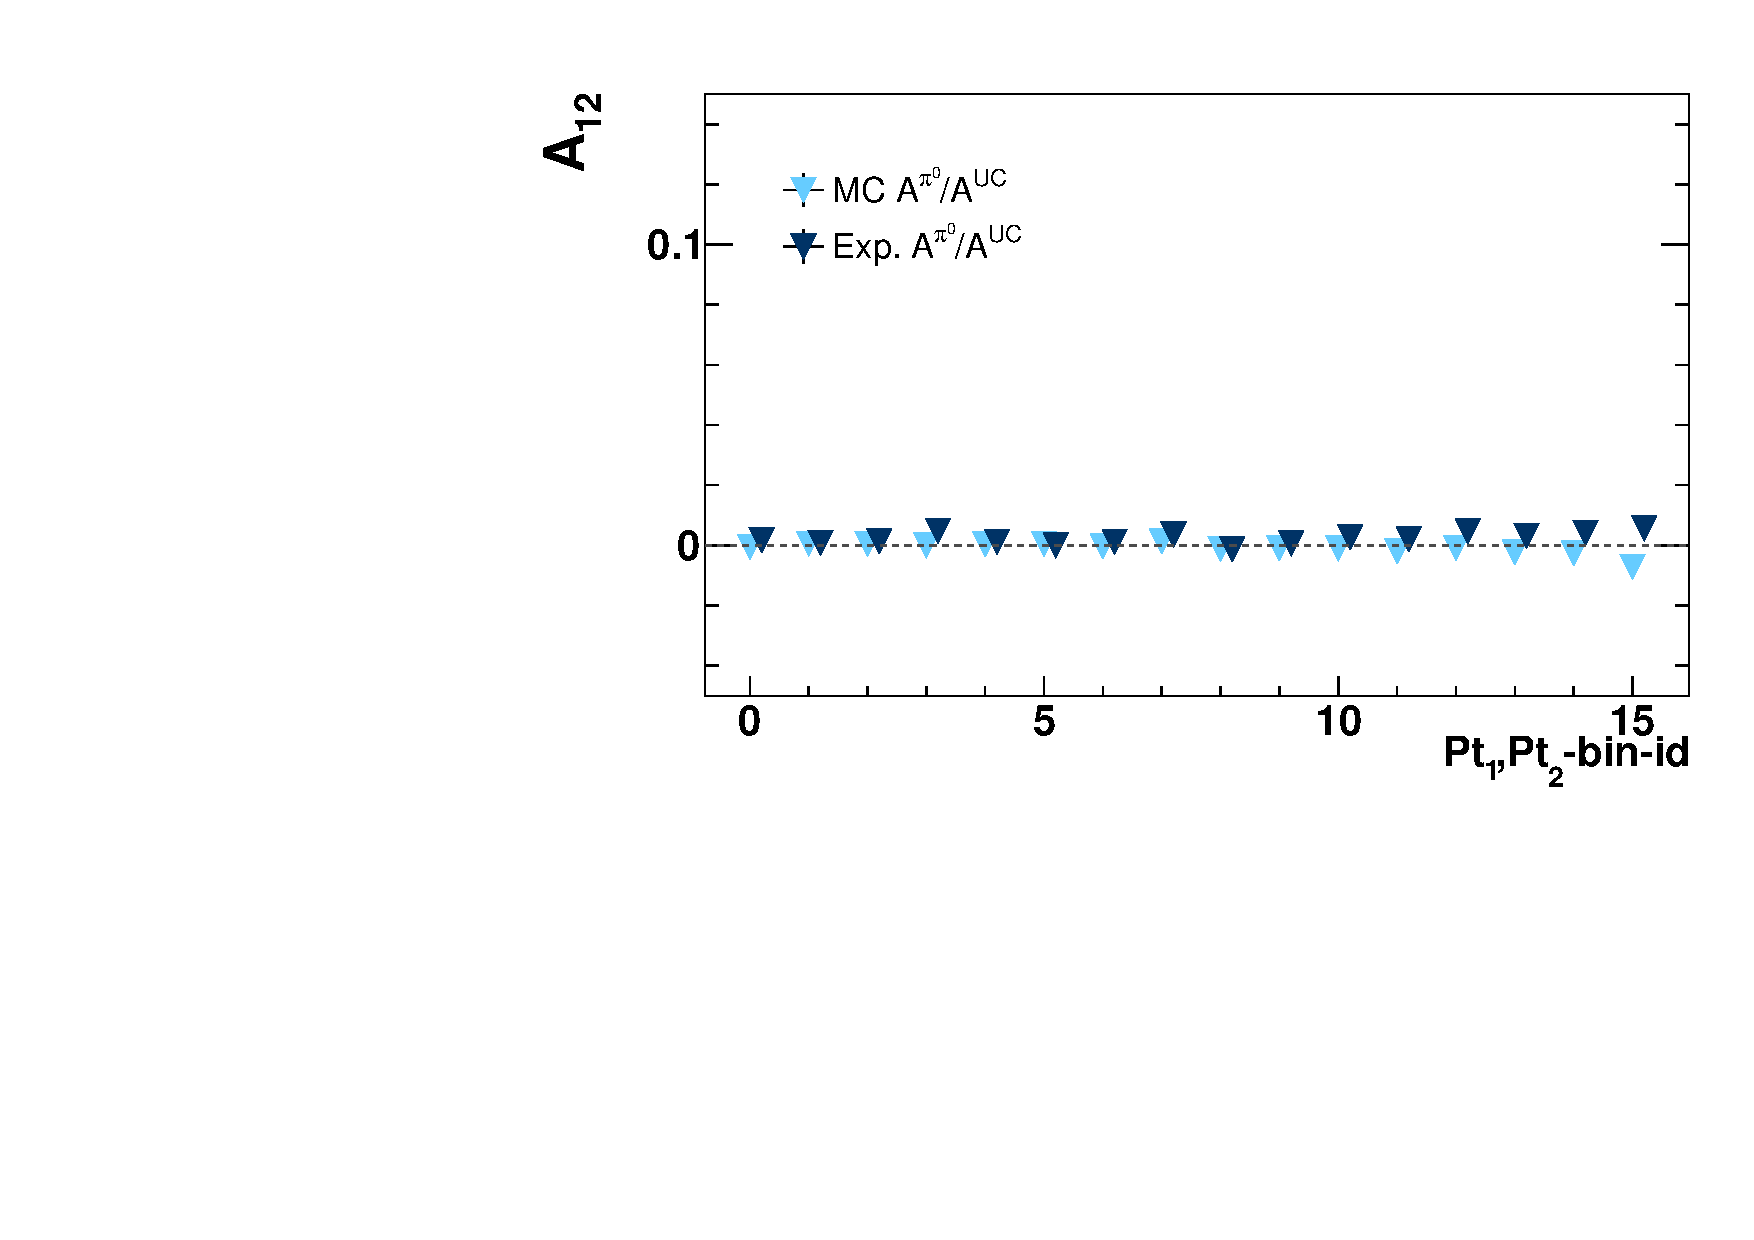
\includegraphics[width=.48\textwidth,natwidth=600,natheight=400]{figure_asy/Pi0OverUC3.pdf}}
  \caption{Double ratio asymmetry $\nicefrac{A^{0\pm}_{12}}{A^C_{12}}$, the dark blue points are from experiment data and the light blue points are MC.}
  \label{fig:exp_pi0_eta_ratio2}
\end{figure}



